% Generated by Sphinx.
\def\sphinxdocclass{report}
\documentclass[letterpaper,10pt]{sphinxmanual}


\usepackage{cmap}
\usepackage[T1]{fontenc}

\usepackage{times}
\usepackage[Sonny]{fncychap}
\usepackage{longtable}
\usepackage{sphinx}
\usepackage{multirow}

     \usepackage{xeCJK}
     \setCJKmainfont{SimSun}
     \XeTeXlinebreaklocale "zh"
     \XeTeXlinebreakskip = 0pt plus 1pt


\title{Linux Documentation}
\date{2015 年 02 月 16 日}
\release{1.0}
\author{wenjian}
\newcommand{\sphinxlogo}{}
\renewcommand{\releasename}{发布}
\makeindex

\makeatletter
\def\PYG@reset{\let\PYG@it=\relax \let\PYG@bf=\relax%
    \let\PYG@ul=\relax \let\PYG@tc=\relax%
    \let\PYG@bc=\relax \let\PYG@ff=\relax}
\def\PYG@tok#1{\csname PYG@tok@#1\endcsname}
\def\PYG@toks#1+{\ifx\relax#1\empty\else%
    \PYG@tok{#1}\expandafter\PYG@toks\fi}
\def\PYG@do#1{\PYG@bc{\PYG@tc{\PYG@ul{%
    \PYG@it{\PYG@bf{\PYG@ff{#1}}}}}}}
\def\PYG#1#2{\PYG@reset\PYG@toks#1+\relax+\PYG@do{#2}}

\expandafter\def\csname PYG@tok@gd\endcsname{\def\PYG@tc##1{\textcolor[rgb]{0.63,0.00,0.00}{##1}}}
\expandafter\def\csname PYG@tok@gu\endcsname{\let\PYG@bf=\textbf\def\PYG@tc##1{\textcolor[rgb]{0.50,0.00,0.50}{##1}}}
\expandafter\def\csname PYG@tok@gt\endcsname{\def\PYG@tc##1{\textcolor[rgb]{0.00,0.27,0.87}{##1}}}
\expandafter\def\csname PYG@tok@gs\endcsname{\let\PYG@bf=\textbf}
\expandafter\def\csname PYG@tok@gr\endcsname{\def\PYG@tc##1{\textcolor[rgb]{1.00,0.00,0.00}{##1}}}
\expandafter\def\csname PYG@tok@cm\endcsname{\let\PYG@it=\textit\def\PYG@tc##1{\textcolor[rgb]{0.25,0.50,0.56}{##1}}}
\expandafter\def\csname PYG@tok@vg\endcsname{\def\PYG@tc##1{\textcolor[rgb]{0.73,0.38,0.84}{##1}}}
\expandafter\def\csname PYG@tok@m\endcsname{\def\PYG@tc##1{\textcolor[rgb]{0.13,0.50,0.31}{##1}}}
\expandafter\def\csname PYG@tok@mh\endcsname{\def\PYG@tc##1{\textcolor[rgb]{0.13,0.50,0.31}{##1}}}
\expandafter\def\csname PYG@tok@cs\endcsname{\def\PYG@tc##1{\textcolor[rgb]{0.25,0.50,0.56}{##1}}\def\PYG@bc##1{\setlength{\fboxsep}{0pt}\colorbox[rgb]{1.00,0.94,0.94}{\strut ##1}}}
\expandafter\def\csname PYG@tok@ge\endcsname{\let\PYG@it=\textit}
\expandafter\def\csname PYG@tok@vc\endcsname{\def\PYG@tc##1{\textcolor[rgb]{0.73,0.38,0.84}{##1}}}
\expandafter\def\csname PYG@tok@il\endcsname{\def\PYG@tc##1{\textcolor[rgb]{0.13,0.50,0.31}{##1}}}
\expandafter\def\csname PYG@tok@go\endcsname{\def\PYG@tc##1{\textcolor[rgb]{0.20,0.20,0.20}{##1}}}
\expandafter\def\csname PYG@tok@cp\endcsname{\def\PYG@tc##1{\textcolor[rgb]{0.00,0.44,0.13}{##1}}}
\expandafter\def\csname PYG@tok@gi\endcsname{\def\PYG@tc##1{\textcolor[rgb]{0.00,0.63,0.00}{##1}}}
\expandafter\def\csname PYG@tok@gh\endcsname{\let\PYG@bf=\textbf\def\PYG@tc##1{\textcolor[rgb]{0.00,0.00,0.50}{##1}}}
\expandafter\def\csname PYG@tok@ni\endcsname{\let\PYG@bf=\textbf\def\PYG@tc##1{\textcolor[rgb]{0.84,0.33,0.22}{##1}}}
\expandafter\def\csname PYG@tok@nl\endcsname{\let\PYG@bf=\textbf\def\PYG@tc##1{\textcolor[rgb]{0.00,0.13,0.44}{##1}}}
\expandafter\def\csname PYG@tok@nn\endcsname{\let\PYG@bf=\textbf\def\PYG@tc##1{\textcolor[rgb]{0.05,0.52,0.71}{##1}}}
\expandafter\def\csname PYG@tok@no\endcsname{\def\PYG@tc##1{\textcolor[rgb]{0.38,0.68,0.84}{##1}}}
\expandafter\def\csname PYG@tok@na\endcsname{\def\PYG@tc##1{\textcolor[rgb]{0.25,0.44,0.63}{##1}}}
\expandafter\def\csname PYG@tok@nb\endcsname{\def\PYG@tc##1{\textcolor[rgb]{0.00,0.44,0.13}{##1}}}
\expandafter\def\csname PYG@tok@nc\endcsname{\let\PYG@bf=\textbf\def\PYG@tc##1{\textcolor[rgb]{0.05,0.52,0.71}{##1}}}
\expandafter\def\csname PYG@tok@nd\endcsname{\let\PYG@bf=\textbf\def\PYG@tc##1{\textcolor[rgb]{0.33,0.33,0.33}{##1}}}
\expandafter\def\csname PYG@tok@ne\endcsname{\def\PYG@tc##1{\textcolor[rgb]{0.00,0.44,0.13}{##1}}}
\expandafter\def\csname PYG@tok@nf\endcsname{\def\PYG@tc##1{\textcolor[rgb]{0.02,0.16,0.49}{##1}}}
\expandafter\def\csname PYG@tok@si\endcsname{\let\PYG@it=\textit\def\PYG@tc##1{\textcolor[rgb]{0.44,0.63,0.82}{##1}}}
\expandafter\def\csname PYG@tok@s2\endcsname{\def\PYG@tc##1{\textcolor[rgb]{0.25,0.44,0.63}{##1}}}
\expandafter\def\csname PYG@tok@vi\endcsname{\def\PYG@tc##1{\textcolor[rgb]{0.73,0.38,0.84}{##1}}}
\expandafter\def\csname PYG@tok@nt\endcsname{\let\PYG@bf=\textbf\def\PYG@tc##1{\textcolor[rgb]{0.02,0.16,0.45}{##1}}}
\expandafter\def\csname PYG@tok@nv\endcsname{\def\PYG@tc##1{\textcolor[rgb]{0.73,0.38,0.84}{##1}}}
\expandafter\def\csname PYG@tok@s1\endcsname{\def\PYG@tc##1{\textcolor[rgb]{0.25,0.44,0.63}{##1}}}
\expandafter\def\csname PYG@tok@gp\endcsname{\let\PYG@bf=\textbf\def\PYG@tc##1{\textcolor[rgb]{0.78,0.36,0.04}{##1}}}
\expandafter\def\csname PYG@tok@sh\endcsname{\def\PYG@tc##1{\textcolor[rgb]{0.25,0.44,0.63}{##1}}}
\expandafter\def\csname PYG@tok@ow\endcsname{\let\PYG@bf=\textbf\def\PYG@tc##1{\textcolor[rgb]{0.00,0.44,0.13}{##1}}}
\expandafter\def\csname PYG@tok@sx\endcsname{\def\PYG@tc##1{\textcolor[rgb]{0.78,0.36,0.04}{##1}}}
\expandafter\def\csname PYG@tok@bp\endcsname{\def\PYG@tc##1{\textcolor[rgb]{0.00,0.44,0.13}{##1}}}
\expandafter\def\csname PYG@tok@c1\endcsname{\let\PYG@it=\textit\def\PYG@tc##1{\textcolor[rgb]{0.25,0.50,0.56}{##1}}}
\expandafter\def\csname PYG@tok@kc\endcsname{\let\PYG@bf=\textbf\def\PYG@tc##1{\textcolor[rgb]{0.00,0.44,0.13}{##1}}}
\expandafter\def\csname PYG@tok@c\endcsname{\let\PYG@it=\textit\def\PYG@tc##1{\textcolor[rgb]{0.25,0.50,0.56}{##1}}}
\expandafter\def\csname PYG@tok@mf\endcsname{\def\PYG@tc##1{\textcolor[rgb]{0.13,0.50,0.31}{##1}}}
\expandafter\def\csname PYG@tok@err\endcsname{\def\PYG@bc##1{\setlength{\fboxsep}{0pt}\fcolorbox[rgb]{1.00,0.00,0.00}{1,1,1}{\strut ##1}}}
\expandafter\def\csname PYG@tok@mb\endcsname{\def\PYG@tc##1{\textcolor[rgb]{0.13,0.50,0.31}{##1}}}
\expandafter\def\csname PYG@tok@ss\endcsname{\def\PYG@tc##1{\textcolor[rgb]{0.32,0.47,0.09}{##1}}}
\expandafter\def\csname PYG@tok@sr\endcsname{\def\PYG@tc##1{\textcolor[rgb]{0.14,0.33,0.53}{##1}}}
\expandafter\def\csname PYG@tok@mo\endcsname{\def\PYG@tc##1{\textcolor[rgb]{0.13,0.50,0.31}{##1}}}
\expandafter\def\csname PYG@tok@kd\endcsname{\let\PYG@bf=\textbf\def\PYG@tc##1{\textcolor[rgb]{0.00,0.44,0.13}{##1}}}
\expandafter\def\csname PYG@tok@mi\endcsname{\def\PYG@tc##1{\textcolor[rgb]{0.13,0.50,0.31}{##1}}}
\expandafter\def\csname PYG@tok@kn\endcsname{\let\PYG@bf=\textbf\def\PYG@tc##1{\textcolor[rgb]{0.00,0.44,0.13}{##1}}}
\expandafter\def\csname PYG@tok@o\endcsname{\def\PYG@tc##1{\textcolor[rgb]{0.40,0.40,0.40}{##1}}}
\expandafter\def\csname PYG@tok@kr\endcsname{\let\PYG@bf=\textbf\def\PYG@tc##1{\textcolor[rgb]{0.00,0.44,0.13}{##1}}}
\expandafter\def\csname PYG@tok@s\endcsname{\def\PYG@tc##1{\textcolor[rgb]{0.25,0.44,0.63}{##1}}}
\expandafter\def\csname PYG@tok@kp\endcsname{\def\PYG@tc##1{\textcolor[rgb]{0.00,0.44,0.13}{##1}}}
\expandafter\def\csname PYG@tok@w\endcsname{\def\PYG@tc##1{\textcolor[rgb]{0.73,0.73,0.73}{##1}}}
\expandafter\def\csname PYG@tok@kt\endcsname{\def\PYG@tc##1{\textcolor[rgb]{0.56,0.13,0.00}{##1}}}
\expandafter\def\csname PYG@tok@sc\endcsname{\def\PYG@tc##1{\textcolor[rgb]{0.25,0.44,0.63}{##1}}}
\expandafter\def\csname PYG@tok@sb\endcsname{\def\PYG@tc##1{\textcolor[rgb]{0.25,0.44,0.63}{##1}}}
\expandafter\def\csname PYG@tok@k\endcsname{\let\PYG@bf=\textbf\def\PYG@tc##1{\textcolor[rgb]{0.00,0.44,0.13}{##1}}}
\expandafter\def\csname PYG@tok@se\endcsname{\let\PYG@bf=\textbf\def\PYG@tc##1{\textcolor[rgb]{0.25,0.44,0.63}{##1}}}
\expandafter\def\csname PYG@tok@sd\endcsname{\let\PYG@it=\textit\def\PYG@tc##1{\textcolor[rgb]{0.25,0.44,0.63}{##1}}}

\def\PYGZbs{\char`\\}
\def\PYGZus{\char`\_}
\def\PYGZob{\char`\{}
\def\PYGZcb{\char`\}}
\def\PYGZca{\char`\^}
\def\PYGZam{\char`\&}
\def\PYGZlt{\char`\<}
\def\PYGZgt{\char`\>}
\def\PYGZsh{\char`\#}
\def\PYGZpc{\char`\%}
\def\PYGZdl{\char`\$}
\def\PYGZhy{\char`\-}
\def\PYGZsq{\char`\'}
\def\PYGZdq{\char`\"}
\def\PYGZti{\char`\~}
% for compatibility with earlier versions
\def\PYGZat{@}
\def\PYGZlb{[}
\def\PYGZrb{]}
\makeatother

\renewcommand\PYGZsq{\textquotesingle}

\begin{document}

\maketitle
\tableofcontents
\phantomsection\label{index::doc}

\begin{quote}\begin{description}
\item[{作者}] \leavevmode
闻健 \href{mailto:wenjianxue2009@live.cn}{wenjianxue2009@live.cn}

\end{description}\end{quote}


\chapter{文章内容:}
\label{index:index}\label{index:id1}\label{index:linux}

\section{Linux网络}
\label{Linux_net/index::doc}\label{Linux_net/index:linux}
主要包括 ipv4和ipv6的配置;arp、ndp的查看;route的配置与查看。


\subsection{IP篇}
\label{Linux_net/ip:ip}\label{Linux_net/ip::doc}

\subsubsection{配置IP}
\label{Linux_net/ip:id1}\begin{description}
\item[{1、 临时配置ipv4地址}] \leavevmode
iconfig

命令格式

ifconfig \textless{}网络接口\textgreater{} \textless{}IP地址\textgreater{} {[}\textless{}netmask 子网掩码\textgreater{} \textless{}broadcast 广播地址\textgreater{}{]}

eg:ifconfig eth0 192.168.0.222

当IP地址使用标准A、B、C类地址时,广播地址和子网掩码可以省略,系统会自动判断广播地址和子网掩码的值并进行设置。否则必须指出广播地址和子网掩码

ifconfig eth0 10.0.0.222 Mask 255.255.255.0 Broadcast 10.0.0.255

1.1 给接口设置多个IP

ifconfig eth0:0 192.168.0.250

ifconfig eth1:0 192.168.1.3

ifconfig eth1:1 192.168.2.3

\begin{notice}{warning}{警告:}
使用 ifconfig 命令设置网络参数会立即生效,但不会修改网络接口配置文件,这将导致所配置的参数在重新启动系统后失效。
\end{notice}

\end{description}

2、永久配置ipv4地址
\begin{quote}

2.1 Redhat系列操作系统

在 /etc/sysconfig/network-scripts 目录下存储网络接口配置文件。每个网络接口有各自的配置文件,配置文件以 ifcfg- 为前缀后接网络接口名。例如,接口 eth0 的配置文件名为 ifcfg-eth0 。
下面是 eth0 接口的配置文件。

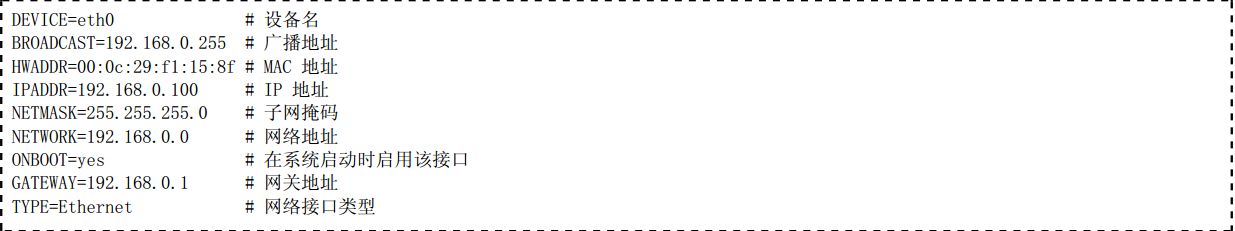
\includegraphics{ifcfg-eth0.png}

您可以根据需要修改此配置文件 ifcfg-eth0 的配置。如果要设置 eth1 的配置文件,您可以复制 ifcfg-eth0 为ifcfg-eth1 然后做适当修改,如果要是为接口配置多个IP地址,可以将ifcfg-eth0拷贝成ifcfg-eth0:0 等,
然后做相应修改

\begin{notice}{warning}{警告:}
修改完成后记得要重启网络服务 service network restart
\end{notice}

2.2 Debian系列操作系统

在/etc/network/interfaces文件中存储着各自接口的配置信息,下图是配置示意,可以根据具体环境设置

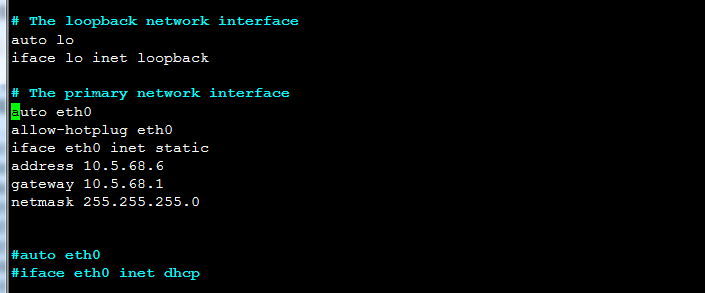
\includegraphics{debian-interface.png}
\end{quote}
\begin{description}
\item[{3、临时配置ipv6地址}] \leavevmode
ifconfig ens33【接口名称】 inet6 add 2001::4/16【ipv6地址】

\item[{4、永久配置ipv6地址}] \leavevmode
在配置文件中输入类似于ipv4的设置

\end{description}


\subsubsection{配置主机名}
\label{Linux_net/ip:id2}
1、临时修改主机名

hostname xxxxx

或

echo xxxxx \textgreater{} /etc/hostname

或

hostname -F /etc/hostname

2、永久修改主机名
\begin{quote}

2.1 Redhat系列操作系统

编辑 /etc/sysconfig/network 文件中的如下配置行:

HOSTNAME=yourhostname

\#将 yourhostname 修改为您的主机名。配置文件修改完毕,在下次重新启动时就会生效。

\begin{notice}{warning}{警告:}
不要忘记还需要修改 /etc/hosts 文件中的主机名。
\end{notice}
\end{quote}


\subsubsection{配置DNS}
\label{Linux_net/ip:dns}
1、修改DNS客户端配置文件

DNS 客户端配置文件为/etc/resolv.conf,使用如下命令添加 DNS 服务器解析的指向。

echo ``nameverver 208.67.222.222'' \textgreater{} /etc/resolv.conf

表示将DNS服务器设置为 208.67.222.222

2、修改 Hosts表 实现静态 DNS 解析

要实现域名解析,即可以使用 DNS 服务器,也可以使用 Hosts表。Hosts表 配置文件是/etc/hosts


\subsubsection{启停网络接口}
\label{Linux_net/ip:id3}
1、启用接口

ifconfig ethx up

2、停用接口

ifconfig  ethx down


\subsubsection{查看网络参数配置}
\label{Linux_net/ip:id4}
1、ifconfig 或者ifconfig -a
\begin{quote}

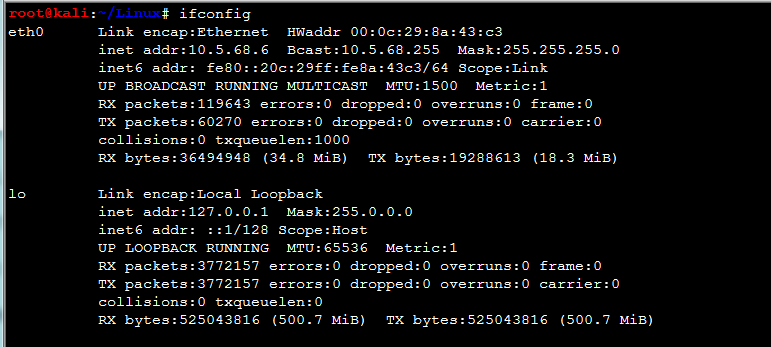
\includegraphics{ifconfig.png}

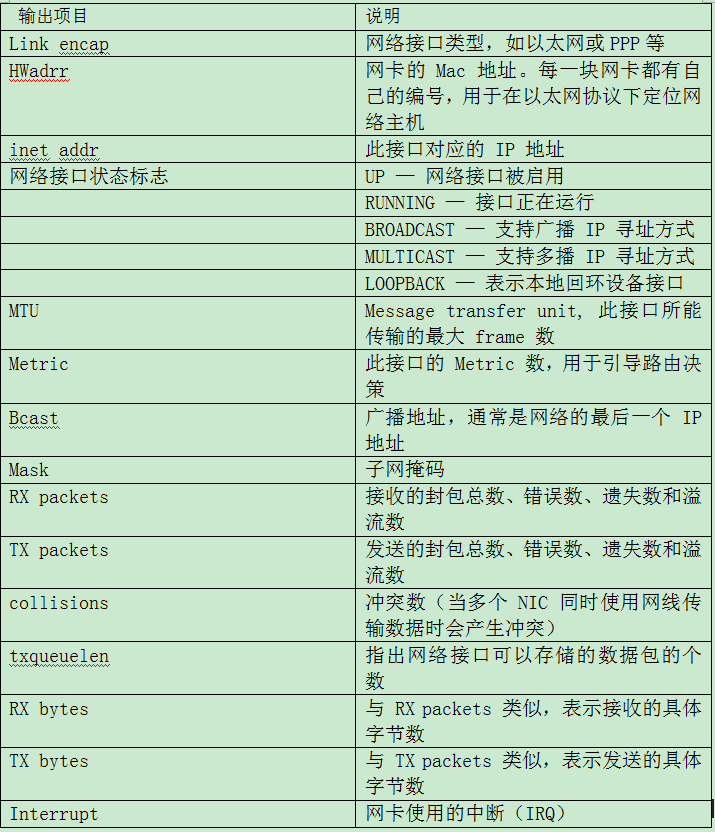
\includegraphics{ifconfig-info.png}
\end{quote}

2、ip address show
\begin{quote}

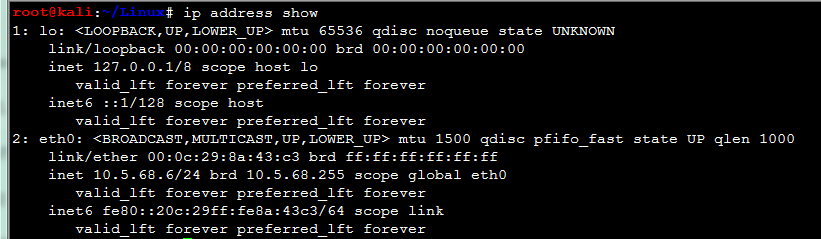
\includegraphics{address-show.png}
\end{quote}

3、ip link list
\begin{quote}

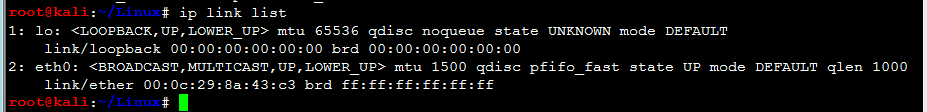
\includegraphics{link-list.png}
\end{quote}


\subsection{ARP篇}
\label{Linux_net/arp:arp}\label{Linux_net/arp::doc}

\subsubsection{Linux 查看arp表项}
\label{Linux_net/arp:linux-arp}
1)arp -a (显示结果比较慢)

2)arp -n

3)ip neigh show (显示的结果较为详细)


\subsubsection{Linux 查看NDP}
\label{Linux_net/arp:linux-ndp}
1)ip -6 neigh show


\subsubsection{Linux 删除arp表项}
\label{Linux_net/arp:id1}
1)ifconfig eth0 down;ifconfig eth0 up

2)ip neigh delete 1.1.1.1 dev eth0

3)arp -d 10.5.68.1


\subsubsection{ARP扫描}
\label{Linux_net/arp:id2}
ARP扫描(ARP请求风暴)

通讯模式(可能):

请求 -\textgreater{} 请求 -\textgreater{} 请求 -\textgreater{} 请求 -\textgreater{} 请求 -\textgreater{} 请求 -\textgreater{} 应答 -\textgreater{} 请求 -\textgreater{} 请求 -\textgreater{} 请求...

描述:

网络中出现大量ARP请求广播包,几乎都是对网段内的所有主机进行扫描。大量的ARP请求广播可能会占用网络带宽资源;ARP扫描一般为ARP攻击的前奏。

出现原因(可能):

{\color{red}\bfseries{}*}病毒程序,侦听程序,扫描程序。

{\color{red}\bfseries{}*}来自和交换机相连的其它主机。


\subsubsection{ARP欺骗防护}
\label{Linux_net/arp:id7}
1、静态绑定

双向绑定

2、使用ARP防护软件

3、定期发送合法的arp应答


\subsubsection{ARP欺骗的防护}
\label{Linux_net/arp:id8}
ARP欺骗和攻击问题,是企业网络的心腹大患。关于这个问题的讨论已经很深入了,
对ARP攻击的机理了解的很透彻,各种防范措施也层出不穷。

但问题是,现在真正摆脱ARP问题困扰了吗?从用户那里了解到,虽然尝试过各种方
法,但这个问题并没有根本解决。原因就在于,目前很多种ARP防范措施,一是解决
措施的防范能力有限,并不是最根本的办法。二是对网络管理约束很大,不方便不实
用,不具备可操作性。三是某些措施对网络传输的效能有损失,网速变慢,带宽浪费
,也不可取。

本节通过具体分析一下普遍流行的四种防范ARP措施,去了解为什么ARP问题始终
不能根治。

上篇:四种常见防范ARP措施的分析

1、双绑措施

双绑是在路由器和终端上都进行IP-MAC绑定的措施,它可以对ARP欺骗的两边,伪
造网关和截获数据,都具有约束的作用。这是从ARP欺骗原理上进行的防范措施,也
是最普遍应用的办法。它对付最普通的ARP欺骗是有效的。

但双绑的缺陷在于3点:

1)在终端上进行的静态绑定,很容易被升级的ARP攻击所捣毁,病毒的一个ARP–d命令,就可以使静态绑定完全失效。

2)在路由器上做IP-MAC表的绑定工作,费时费力,是一项繁琐的维护工作。换个网卡或更换IP,都需要重新配置路由。对于流动性电脑,这个需要随时进行的绑定工作,是网络维护的巨大负担,网管员几乎无法完成。

3)双绑只是让网络的两端电脑和路由不接收相关ARP信息,但是大量的ARP攻击数据还是能发出,还要在内网传输,大幅降低内网传输效率,依然会出现问题。

因此,虽然双绑曾经是ARP防范的基础措施,但因为防范能力有限,管理太麻烦,现在它的效果越来越有限了。

2、ARP个人防火墙

在一些杀毒软件中加入了ARP个人防火墙的功能,它是通过在终端电脑上对网关进行
绑定,保证不受网络中假网关的影响,从而保护自身数据不被窃取的措施。ARP防火
墙使用范围很广,有很多人以为有了防火墙,ARP攻击就不构成威胁了,其实完全不
是那么回事。

ARP个人防火墙也有很大缺陷:

1)它不能保证绑定的网关一定是正确的。如果一个网络中已经发生了ARP欺骗,有
人在伪造网关,那么,ARP个人防火墙上来就会绑定这个错误的网关,这是具有极大
风险的。即使配置中不默认而发出提示,缺乏网络知识的用户恐怕也无所适从。

2)ARP是网络中的问题,ARP既能伪造网关,也能截获数据,是个“双头怪”。在
个人终端上做ARP防范,而不管网关那端如何,这本身就不是一个完整的办法。AR
P个人防火墙起到的作用,就是防止自己的数据不会被盗取,而整个网络的问题,如
掉线、卡滞等,ARP个人防火墙是无能为力的。

因此,ARP个人防火墙并没有提供可靠的保证。最重要的是,它是跟网络稳定无关的
措施,它是个人的,不是网络的。

3、VLAN和交换机端口绑定

通过划分VLAN和交换机端口绑定,以图防范ARP,也是常用的防范方法。做法是细
致地划分VLAN,减小广播域的范围,使ARP在小范围内起作用,而不至于发生大面
积影响。同时,一些网管交换机具有MAC地址学习的功能,学习完成后,再关闭这
个功能,就可以把对应的MAC和端口进行绑定,避免了病毒利用ARP攻击篡改自身
地址。也就是说,把ARP攻击中被截获数据的风险解除了。这种方法确实能起到一定
的作用。

不过,VLAN和交换机端口绑定的问题在于:

1)、没有对网关的任何保护,不管如何细分VLAN,网关一旦被攻击,照样会造成全
网上网的掉线和瘫痪。

2)把每一台电脑都牢牢地固定在一个交换机端口上,这种管理太死板了。这根本不
适合移动终端的使用,从办公室到会议室,这台电脑恐怕就无法上网了。在无线应用
下,又怎么办呢?还是需要其他的办法。

3)实施交换机端口绑定,必定要全部采用高级的网管交换机、三层交换机,整个交
换网络的造价大大提高。

因为交换网络本身就是无条件支持ARP操作的,就是它本身的漏洞造成了ARP攻击
的可能,它上面的管理手段不是针对ARP的。因此,在现有的交换网络上实施ARP
防范措施,属于以子之矛攻子之盾。而且操作维护复杂,基本上是个费力不讨好的事
情。

4、PPPoE

网络下面给每一个用户分配一个帐号、密码,上网时必须通过PPPoE认证,这种方
法也是防范ARP措施的一种。PPPoE拨号方式对封包进行了二次封装,使其具备了
不受ARP欺骗影响的使用效果,很多人认为找到了解决ARP问题的终极方案。

问题主要集中在效率和实用性上面:

1)PPPoE需要对封包进行二次封装,在接入设备上再解封装,必然降低了网络传输
效率,造成了带宽资源的浪费,要知道在路由等设备上添加PPPoE Server的处理效
能和电信接入商的PPPoE Server可不是一个数量级的。

2)PPPoE方式下局域网间无法互访,在很多网络都有局域网内部的域控服务器、D
NS服务器、邮件服务器、OA系统、资料共享、打印共享等等,需要局域网间相互通
信的需求,而PPPoE方式使这一切都无法使用,是无法被接受的。

3)不使用PPPoE,在进行内网访问时,ARP的问题依然存在,什么都没有解决,网
络的稳定性还是不行。

因此,PPPoE在技术上属于避开底层协议连接,眼不见心不烦,通过牺牲网络效率
换取网络稳定。最不能接受的,就是网络只能上网用,内部其他的共享就不能在PPP
oE下进行了。

通过对以上四种普遍的ARP防范方法的分析,我们可以看出,现有ARP防范措施都
存在问题。这也就是ARP即使研究很久很透,但依然在实践中无法彻底解决的原因所
在了。

下篇:免疫网络是解决ARP最根本的办法

道高一尺魔高一丈,网络问题必定需要网络的方法去解决。目前,欣全向推广的免疫
网络就是彻底解决ARP问题的最实际的方法。

从技术原理上,彻底解决ARP欺骗和攻击,要有三个技术要点。

1)终端对网关的绑定要坚实可靠,这个绑定能够抵制被病毒捣毁。

2)接入路由器或网关要对下面终端IP-MAC的识别始终保证唯一准确。

3)网络内要有一个最可依赖的机构,提供对网关IP-MAC最强大的保护。它既能够分
发正确的网关信息,又能够对出现的假网关信息立即封杀。

免疫网络在这三个问题上,都有专门的技术解决手段,而且这些技术都是厂家欣全向
的技术专利。下面我们会详细说明。现在,我们要先做一个免疫网络结构和实施的简
单介绍。

免疫网络就是在现有的路由器、交换机、网卡、网线构成的普通交换网络基础上,加
入一套安全和管理的解决方案。这样一来,在普通的网络通信中,就融合进了安全和
管理的机制,保证了在网络通信过程中具有了安全管控的能力,堵上了普通网络对安
全从不设防的先天漏洞。

免疫网络的结构

实施一个免疫网络不是一个很复杂的事,代价并不大。它要做的仅仅是用免疫墙路由
器或免疫网关,替换掉现有的宽带接入设备。在免疫墙路由器下,需要自备一台服务
器24小时运行免疫运营中心。免疫网关不需要,已自带服务器。这就是方案的所需
要的硬件调整措施。

软性的网络调整是IP规划、分组策略、终端自动安装上网驱动等配置和安装工作,以
保证整个的安全管理功能有效地运行。其实这部分工作和网管员对网络日常的管理没
有太大区别。

免疫网络的监控中心

免疫网络具有强大的网络基础安全和管理功能,对ARP的防范仅是其十分之一不到的
能力。但本文谈的是ARP问题,所以我们需要回过头来,具体地解释免疫网络对AR
P欺骗和攻击防范的机理。至于免疫网络更多的强大,可以后续研究。

前述治理ARP问题的三个技术要点,终端绑定、网关、机构三个环节,免疫网络分别
采用了专门的技术手段。

1)终端绑定采用了看守式绑定技术。免疫网络需要每一台终端自动安装驱动,不安
装或卸载就不能上网。在驱动中的看守式绑定,就是把正确的网关信息存贮在非公开
的位置加以保护,任何对网关信息的更改,由于看守程序的严密监控,都是不能成功
的,这就完成了对终端绑定牢固可靠的要求。

2)免疫墙路由器或免疫网关的ARP先天免疫技术。在NAT转发过程中,由于加入了
特殊的机制,免疫墙路由器根本不理会任何对终端IP-MAC的ARP申告,也就是说,
谁都无法欺骗网关。与其他路由器不同,免疫墙路由器没有使用IP-MAC的列表进行
工作,当然也不需要繁琐的路由器IP-MAC表绑定和维护操作。先天免疫,就是不用
管也具有这个能力。

3)保证网关IP-MAC始终正确的机构,在免疫网络中是一套安全机制。首先,它能够
做到把从路由器中取到的真实网关信息,分发到每一个网内终端,而安装有驱动的终
端,只接受这样的信息,其他信息不能接受,保证了网关的唯一正确性。其次,在每
一台终端,免疫驱动都会拦截病毒发出的错误网关传播,不使其流窜到网络内


\subsubsection{负载均衡三角传输(DR)模式之ARP禁止响应}
\label{Linux_net/arp:dr-arp}
echo ``1'' \textgreater{}/proc/sys/net/ipv4/conf/lo/arp\_ignore

echo ``2'' \textgreater{}/proc/sys/net/ipv4/conf/lo/arp\_announce

echo ``1'' \textgreater{}/proc/sys/net/ipv4/conf/all/arp\_ignore

echo ``2'' \textgreater{}/proc/sys/net/ipv4/conf/all/arp\_announce

/sbin/route add -host \$VIP dev lo:0


\subsection{路由篇}
\label{Linux_net/route::doc}\label{Linux_net/route:id1}

\subsubsection{查看Linux 内核路由(ipv4)}
\label{Linux_net/route:linux-ipv4}
1)route

或

route -n

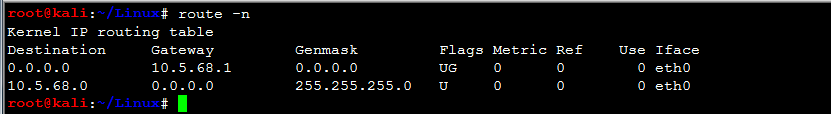
\includegraphics{kernel-route.png}

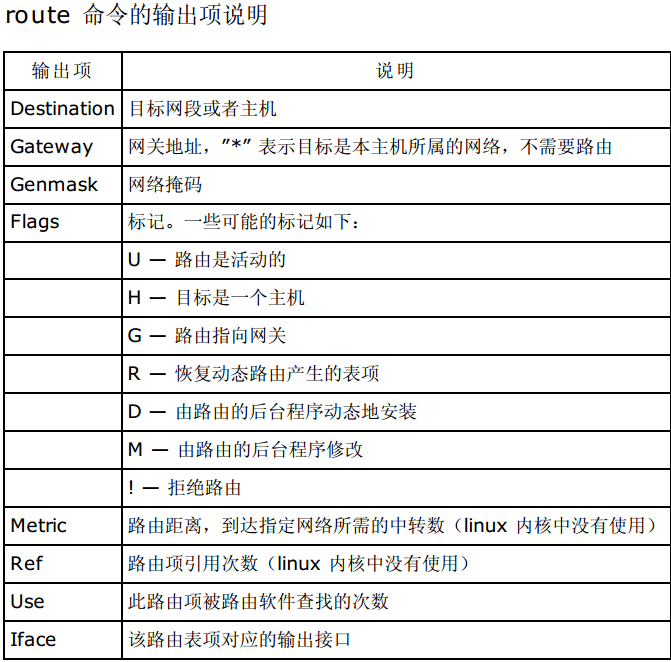
\includegraphics{route.png}

2)ip route show


\includegraphics{route-show.png}

3)ip route list table local
\begin{quote}

ip route list table main
\end{quote}

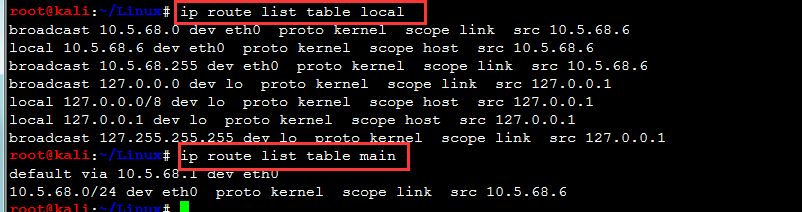
\includegraphics{table-local.png}


\subsubsection{查看Linux 内核路由(ipv6)}
\label{Linux_net/route:linux-ipv6}
1)route -n -6

2)route -A inet6

3)ip -6 route show

4)ip -6 route show dev eth0


\subsubsection{添加路由(ipv4)}
\label{Linux_net/route:ipv4}
添加默认路由

1)ip route add default via 10.5.68.1 dev eth0 table test

添加到主机的路由

2)route add -host 192.168.1.2 dev eth0:0

3)route add -host 10.20.30.148 gw 10.20.30.40

添加到网络的路由

4)route add -net 10.20.30.40 netmask 255.255.255.248 eth0

5)route add -net 10.20.30.48 netmask 255.255.255.248 gw 10.20.30.41

6)route add -net 192.168.1.0/24 eth1


\subsubsection{添加路由(ipv6)}
\label{Linux_net/route:ipv6}
1)ip -6 route add 2000::/3 via 3ffe:ffff:0:f101::1

2)route -A inet6 add 2000::/3 gw 3ffe:ffff:0:f101::1

3)ip -6 route add 2000::/3 dev eth0 metric 1

4)route -A inet6 add 2000::/3 dev eth0

5)route -A inet6 add default gw 2001:250:3000:2:2c0:95ff:fee0:473f


\subsubsection{删除路由(ipv4)}
\label{Linux_net/route:id2}
1)route del -host 192.168.1.2 dev eth0:0

2)route del -host 10.20.30.148 gw 10.20.30.40

3)route del -net 10.20.30.40 netmask 255.255.255.248 eth0

4)route del -net 10.20.30.48 netmask 255.255.255.248 gw 10.20.30.41

5)route del -net 192.168.1.0/24 eth1

6)route del default gw 192.168.1.1


\subsubsection{删除路由(ipv6)}
\label{Linux_net/route:id3}
1)ip -6 route del 2000::/3 via 3ffe:ffff:0:f101::1

2)route -A inet6 del 2000::/3 gw 3ffe:ffff:0:f101::1

3)ip -6 route del 2000::/3 dev eth0

4)route -A inet6 del 2000::/3 dev eth0


\subsubsection{刷新路由表}
\label{Linux_net/route:id4}
ip route flush  cache


\subsubsection{三种路由类型}
\label{Linux_net/route:id5}
主机路由

主机路由是路由选择表中指向单个IP地址或主机名的路由记录。主机路由的Flags字段为H。例如,在下面的示例中,
本地主机通过IP地址192.168.1.1的路由器到达IP地址为10.0.0.10的主机。

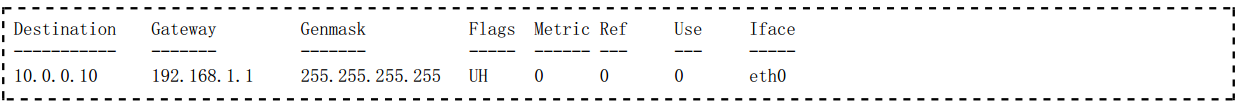
\includegraphics{host-route.png}

网络路由

网络路由是代表主机可以到达的网络。网络路由的Flags字段为N。例如,在下面的示例中,本地主机将发送到网络
192.19.12的数据包转发到IP地址为192.168.1.1的路由器。

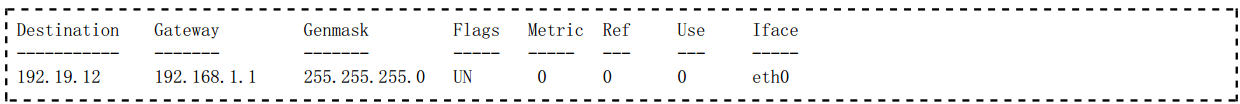
\includegraphics{network-route.png}

默认路由

当主机不能在路由表中查找到目标主机的IP地址或网络路由时,数据包就被发送到默认路由(默认网关)上。默认路由
的Flags字段为G。例如,在下面的示例中,默认路由是IP地址为192.168.1.1的路由器。

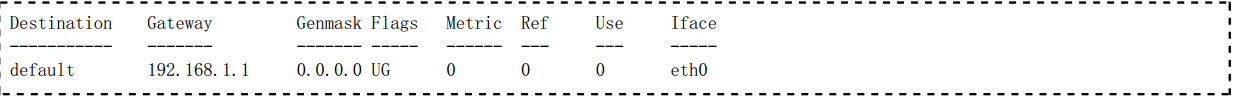
\includegraphics{default-route.png}


\subsubsection{设置路由转发}
\label{Linux_net/route:id6}
1)临时生效

echo `1' \textgreater{}/proc/sys/net/ipv4/ip\_forward

\begin{notice}{warning}{警告:}
重启后配置失效
\end{notice}

2)永久生效

sysctl -w net.ipv4.ip\_forward=1

或

echo ``net.ipv4.ip\_forward = 1'' \textgreater{}\textgreater{}/etc/sysctl.conf

\begin{notice}{warning}{警告:}
别忘记使用 sysctl -p 是配置生效
\end{notice}

3)查看系统目前支不支持路由转发

sysctl net.ipv4.ip\_forward


\section{Linux查找\textbar{}过滤命令}
\label{Linux_find/index::doc}\label{Linux_find/index:linux}
1、文件查找 (find、locate)

2、内容查找  (grep)

3、内容过滤(cat、cut、tail、head)


\subsection{文件查找}
\label{Linux_find/file::doc}\label{Linux_find/file:id1}

\subsubsection{find}
\label{Linux_find/file:find}
\textbf{1、find 命令的格式}

find 命令用于在文件系统中查找满足条件的文件。find 命令功能强大,提供了相当多的查找条件。find 命令还可以对查找到的文件做操作,如执行
Shell 命令等。

find 命令的格式是:

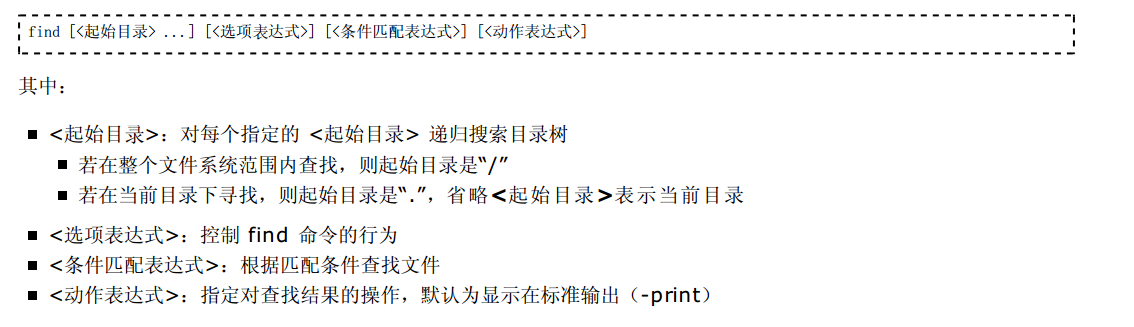
\includegraphics{findformat.png}

不带任何参数的 find 命令将在屏幕上递归显示当前目录下的文件列表。下面给出一些常用的表达式的解释。

\textbf{2、选项表达式}

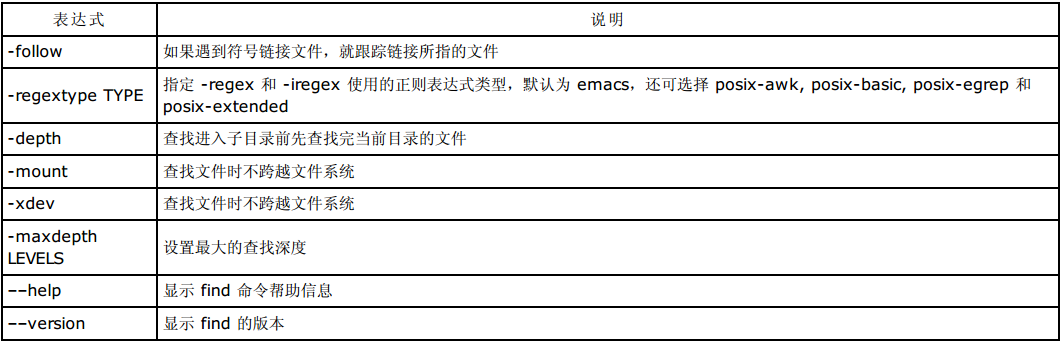
\includegraphics{options.png}

\textbf{3、条件匹配表达式}


\includegraphics{condition.png}

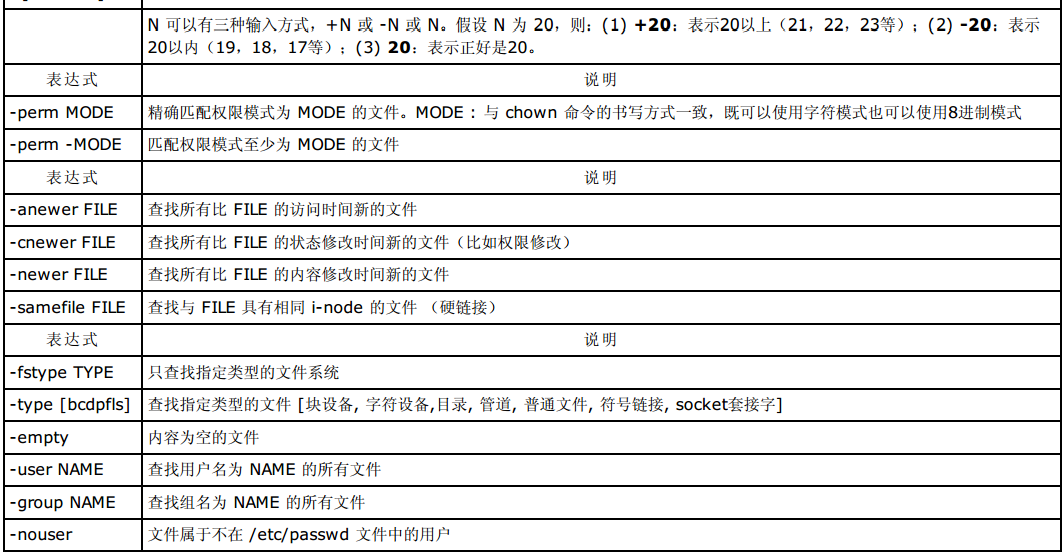
\includegraphics{condition2.png}


\includegraphics{condition3.png}

\textbf{4、动作表达式}

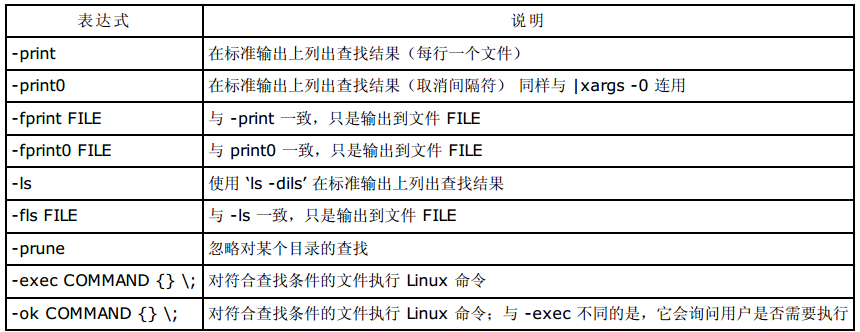
\includegraphics{action.png}

\textbf{5、组合条件表达式}

在书写表达式时,可以使用逻辑运算符与、或、非组成的复合条件,并可以用()改变默认的操作符优先级。下面以优先
级由高到低列出可用的逻辑操作符。若以空格作为各个表达式的间隔符,则各个表示式之间是与关系。

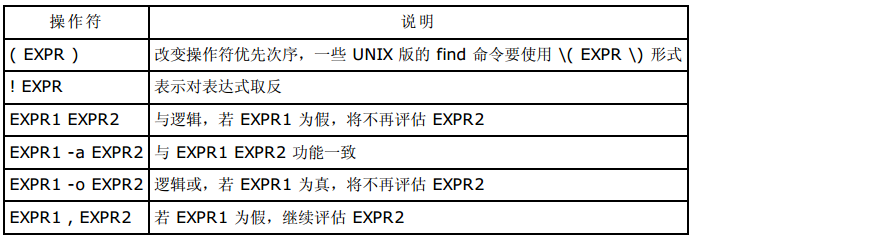
\includegraphics{combine.png}

\textbf{6、find 命令使用举例}

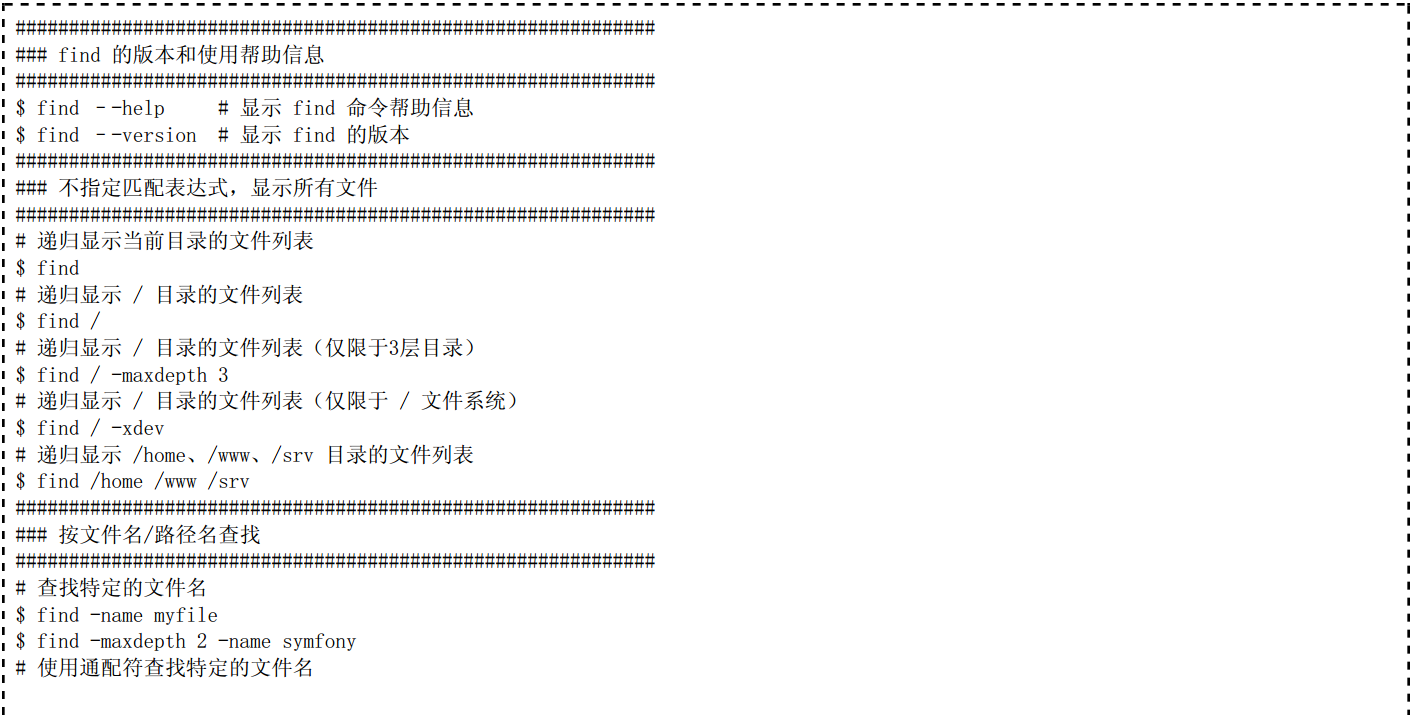
\includegraphics{eg1.png}


\includegraphics{eg2.png}

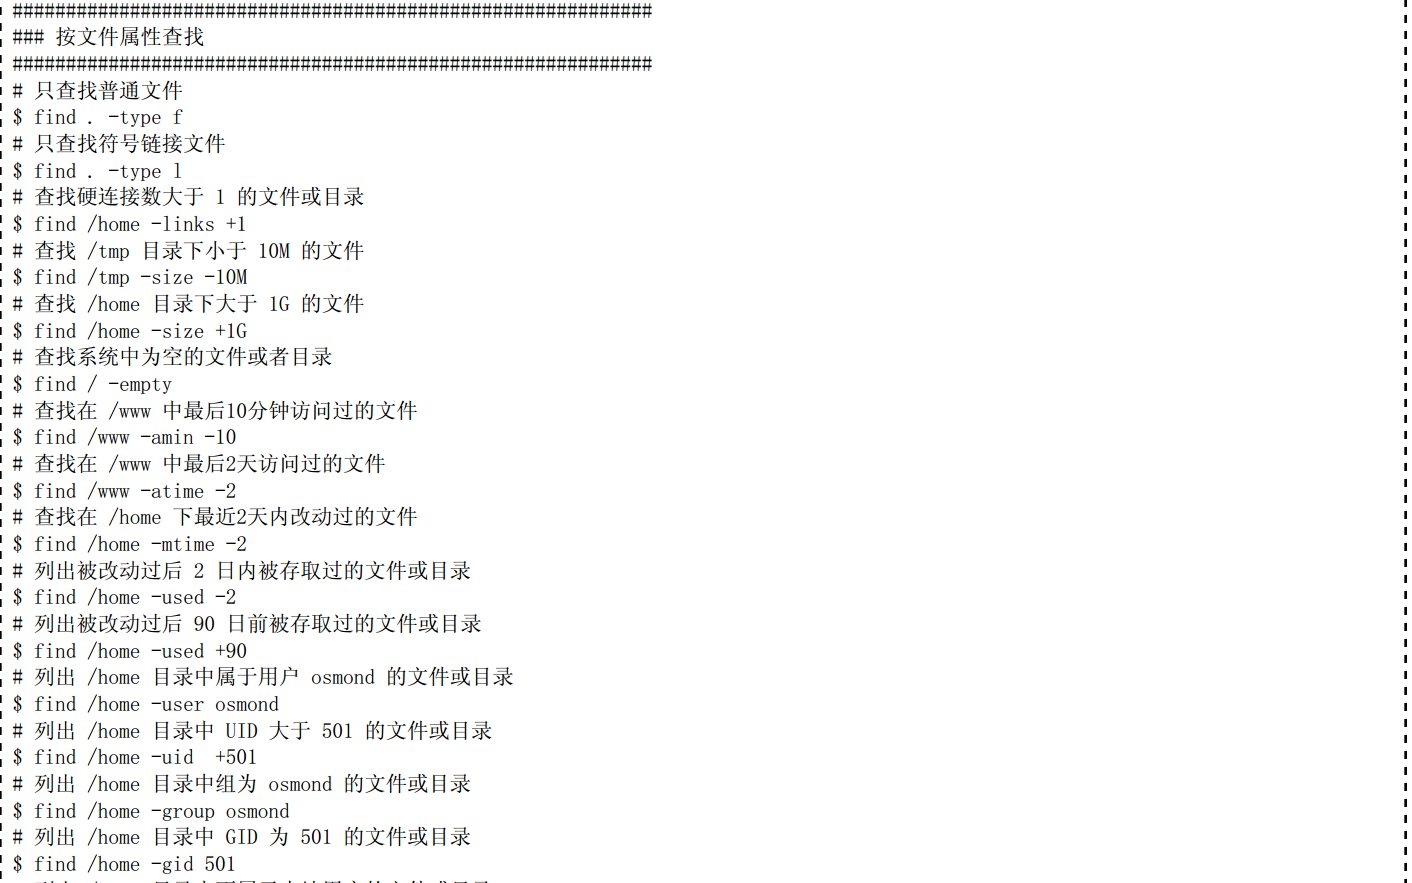
\includegraphics{eg3.png}


\includegraphics{eg4.png}

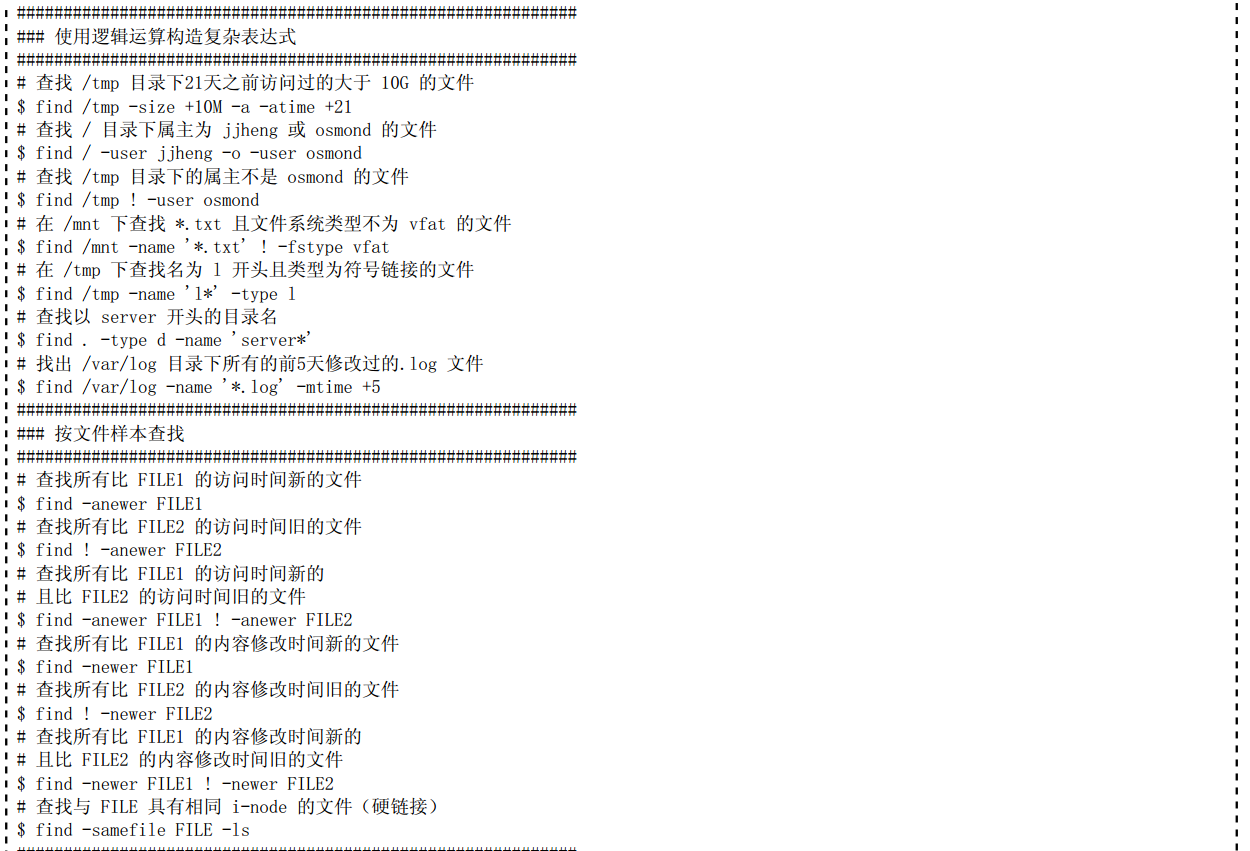
\includegraphics{eg5.png}

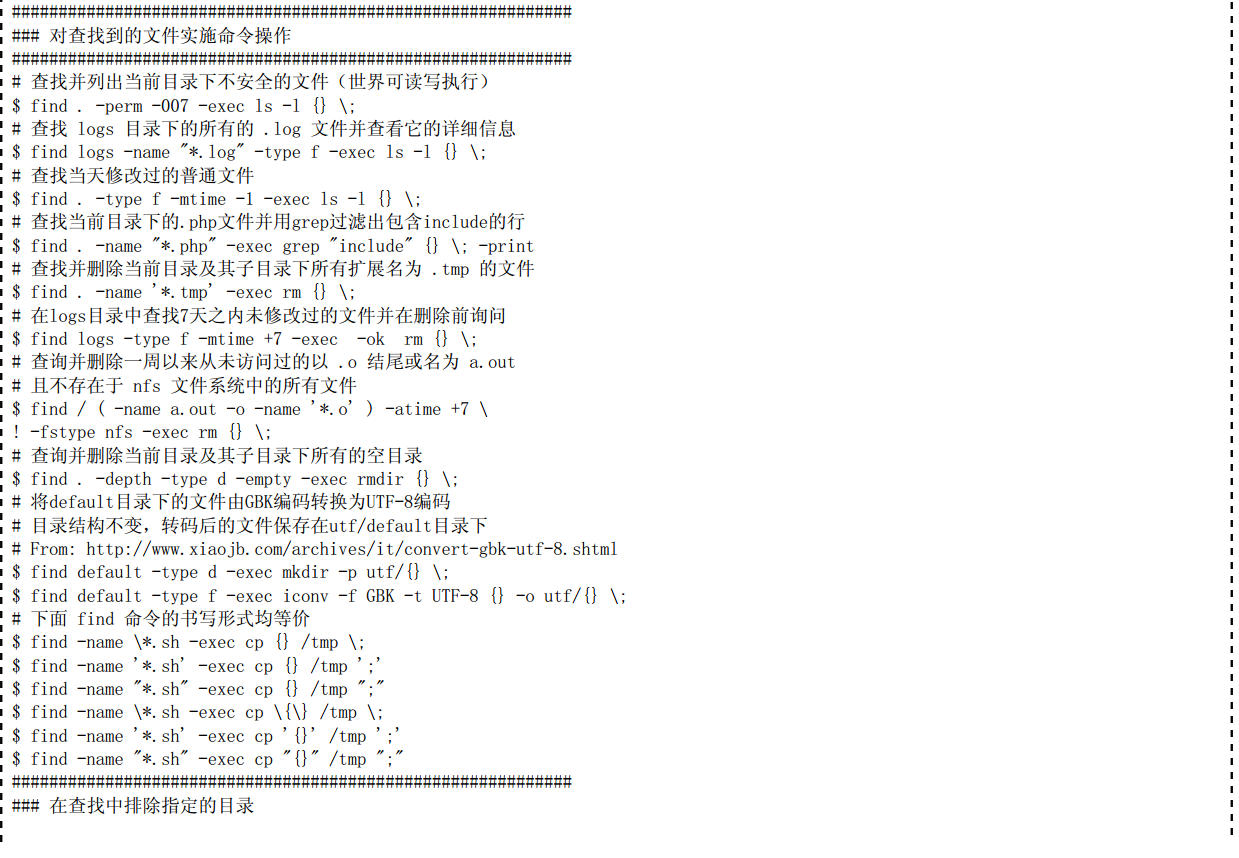
\includegraphics{eg6.png}

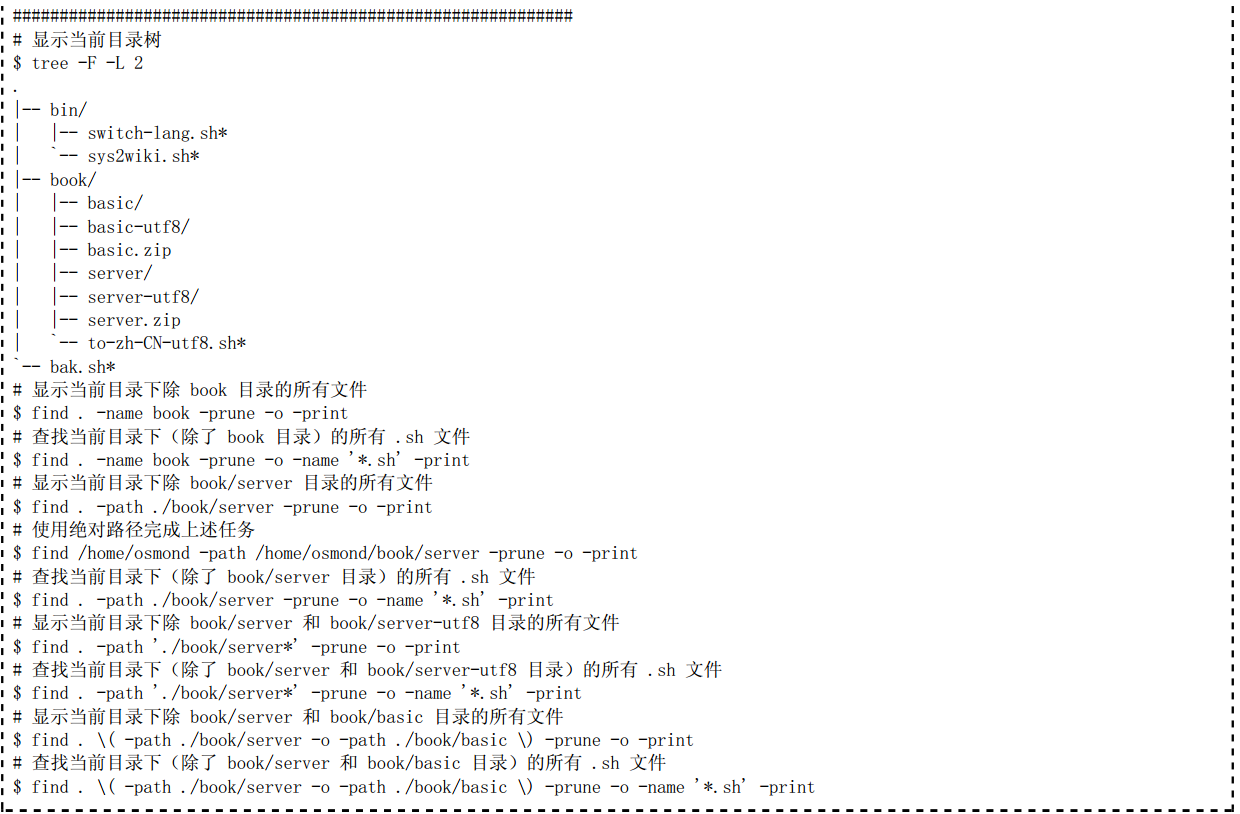
\includegraphics{eg7.png}

1)find ./ -type f -name ``{\color{red}\bfseries{}*}.txt'' {\color{red}\bfseries{}\textbar{}}xargs -i cp \{\} tmp/

2)用shell查询以“.”结尾的文件,并加上后缀“.ts”

find ./ -name ``{\color{red}\bfseries{}*}.'' exec mv \{\} \{\}ats ;

3)查找所有具有suid的文件
\begin{quote}

find / -perm -4100 -exec ls -l \{\} ;

find / -type f -perm -u=s
\end{quote}

4)查找所有sgid的文件

find / -perm -2010 -exec ls -l \{\} ;

5)查找同时具有suid和sgid属性的文件

find / -perm -6110 -exec ls -l \{\} ;

6)find . -type f -perm 6000   \#完全匹配

find . -type f -perm -6000  \#有1的位置必须一样

find . -type f -perm +6000  \#只要有其中一个有1的匹配就行

这些8进制的权限对比的时候要换成2进制形式)

7)查找含有sgid权限位的目录

find / -type f or type d -perm 2000

find / -type f or type d -perm -g=s

8)查找含有tickty权限位的目录

find / -type d -perm 1000

9)查看危险目录

find / -perm -222 -type d

find / -perm -o+w -tye d


\subsubsection{Locate}
\label{Linux_find/file:locate}
locate -r ``ls\$''

locate -r ``\textasciicircum{}ls''

locate -r `\textasciicircum{}/bin.*ls\$'

locate -r `.*/bin.*\textless{}passwd\$'  \#\textless{}passwd 表示以passwd单词开头

locate -r `.*/bin.*\textless{}passwd\textgreater{}'  \#包含passwd单词即可


\subsection{内容查找与过滤}
\label{Linux_find/content::doc}\label{Linux_find/content:id1}

\subsubsection{cut}
\label{Linux_find/content:cut}
功能说明: 纵向切割出文本指定的部分并写到标准输出,显示文件或STDIN数据的指定列

使用 -d 指定区分列的定界符(默认为TAB)

使用 -f 指定要显示的列

\$ cut -d: -f1 /etc/passwd (默认的分隔符是tab)

\$ grep root /etc/passwd \textbar{} cut -d: -f7

使用 -c 按字符切割
\$ cut -c2-5 /usr/share/dict/words

-s : 不打印没有包含分界符的行 (默认的分解符为tab,可以使用-d参数修改)

-b\textless{}LIST\textgreater{} : 只列出\textless{}LIST\textgreater{}指定的字节

-c\textless{}LIST\textgreater{} : 只列出\textless{}LIST\textgreater{}指定的字符

1、cut -b-10 file \#只列出每行的开头到第10个字节的内容

2、cut -b2-10  \#列出每行第2到第10的字节的内容

3、cut -b2-10,15-20  \#列出每行第2到第10的字节,15到20字节的内容

4、cut -c5- file  \#列出每行第5个字符到最后的所有内容

5、cut -c5-10 file \#列出每行第2到第10的字符的内容

6、cut -c5-10,15-20 file \#列出每行5到10字符,15到20字符的内容

7、cut -f1,3,5 file  \#列出每行1、3、5字段的内容

8、cut -f2-4 file  \#列出每行2到4字段的内容

9、cut -f1,2-4,6 -d' ` -s file

10、cut命令-d不能和-c一起用

11、cut -b8 file  \#列出每一行的第8个字节的内容


\subsubsection{grep}
\label{Linux_find/content:grep}
1、grep -R `10.1.198.85' /etc \#-R表示目录递归

2、grep `test' d*  \#显示所有以d开头的文件中包含 test的行

3、grep ‘test’ aa bb cc    \#显示在aa,bb,cc文件中包含test的行

4、grep magic /usr/src  \#显示/usr/src目录下的文件(不含子目录)包含magic的行

5、grep -r magic /usr/src  \#显示/usr/src目录下的文件(包含子目录)包含magic的行

6、grep -w pattern files :只匹配整个单词,而不是字符串的一部分(如匹配’magic’,而不是’magical’),

7、grep ‘{[}a-z{]}\{5\}’ aa \#显示所有包含每行字符串至少有5个连续小写字符的字符串的行

8、grep -v -E `grep\textbar{}monitor' /etc/passwd \#过滤掉含有grep或者monitor的行

9、-n 可以打印匹配行的行号 显示的结果后面为行号: xxxx (xxx为匹配行的内容)

10、-s 表示不打印错误信息,但是正常的匹配成功信息还是会打印的,而-q则是什么都不打印

grep 的其他参数

-i 表示不区分大小写

-v 表示匹配的但不显示

11、grep -c china  dict.txt  \# 统计包含china的行数

ps -ef {\color{red}\bfseries{}\textbar{}}grep -A2 -B2 wenjian \#显示匹配行和匹配上的上2两行,下两行

12、grep ``{\color{red}\bfseries{}*}test''  example.txt \#这里面的通配符*不能被grep正确处理,grep默认不识别通配符,只好加行-E选项

13、grep test example.txt

grep test \textless{}example.txt

cat example.txt  \textbar{} grep test

\#以上三个都是等效的,grep可以处理管道输入也可以处理标准输入

14、cat test.sh \textbar{} grep -n `echo'
\begin{quote}

5:    echo ``very good!''
\end{quote}
\begin{description}
\item[{;}] \leavevmode
7:    echo ``good!'';

9:    echo ``pass!'';

11:    echo ``no pass!'';

\end{description}

\#grep 过滤后输出的行号是原始内容的行号,没有发生改变

15、标准输入优于管道输入
sed -n `1,10p'\textless{}test.sh \textbar{} grep -n `echo' \textless{}testsh.sh

10:echo \$total;

18:echo \$total;

21:     echo ``ok'';

\#哈哈,这个grep又接受管道输入,又有testsh.sh输入,那是不是2个都接收呢。刚才说了''\textless{}''运算符会优先,管道还没有发送数据前,grep绑定了testsh.sh输入,这样sed命令输出就被抛弃了。这里一定要小心使用

16、grep 使用 Basic regular expression (BR E) 书写匹配模式

egrep 使用 Extended regular expression (ER E) 书写匹配模式,等效于 grep -E

fgrep 不使用任何正则表达式书写匹配模式(以固定字符串对待),执行快速搜索,等效于 grep -F

17、grep -v `\textasciicircum{}\#' myfile

18、grep `{[}a-z{]}\{5\}' myfile

19、egrep `{[}a-z{]}\{5\}' myfile

20、\# 如果west被匹配,则es就被存储到内存中,并标记为1,然后搜索任意个字符(.*),

\# 这些字符后面紧跟着另外一个es(1),找到就显示该行。

grep `w(es)t.*1' myfile

egrep `w(es)t.*1' myfile

21、通过管道过滤ls输出的内容,只显示以 \textasciitilde{} 或 - 或 .bak 结尾的行
\begin{quote}

ls \textbar{} egrep `(\textasciitilde{}\textbar{}-{\color{red}\bfseries{}\textbar{}}.bak)\$'
\end{quote}


\subsubsection{tr}
\label{Linux_find/content:tr}

\subsubsection{other}
\label{Linux_find/content:other}
1、cat -n text.sql

-n:由 1 开始对所有输出的行进行编号

2、cat -b text.sql

-b : 和 -n 相似,只不过对于空行不编号

3、cat -b -s text.sql

-s : 当遇到有连续两行以上的空行时,使用一个空行代替

4、cat file1 file2 \textgreater{} files

将两个文件内容合并

Linux tail

tail 命令从指定点开始将 File 参数指定的文件写到标准输出。如果没有指定文件,则会使用标准输入
默认在标准输出上显示每个FILE的最后10行. 如果多于一个FILE,会一个接一个地显示, 并在每个文件显示的首部给出文件名. 如果没有FILE,或者FILE是-,那么就从标准输入上读取.

tail /etc/passwd 查看passwd文件后十行的内容

tail -2 /etc/passwd  查看passwd文件后两行内容

tail -f /etc/passwd  实时查看passwd文件后十行内容

tail - 表示从标准终输入读取

tail -n 20 /etc/passwd 显示最后20行的内容

tail -c 10 /etc/passwd 显示passwd最后10个字节

more +10 file1

从第10行开始向下显示内容


\section{Linux Log}
\label{Linux_log/index::doc}\label{Linux_log/index:linux-log}
日志是安全事件、异常事件分析的入口,打好日志分析基础很重要


\subsection{syslog}
\label{Linux_log/syslog:syslog}\label{Linux_log/syslog::doc}

\subsubsection{日志系统}
\label{Linux_log/syslog:id1}
\textbf{1、什么是 syslog}

日志的主要用途是系统审计、监测追踪和分析统计。

为了保证 Linux 系统正常运行、准确解决遇到的各种各样的系统问题,认真地读取日志文件是管理员的一项非常重要的
任务。

Linux 内核由很多子系统组成,包括网络、文件访问、内存管理等。子系统需要给用户传送一些消息,这些消息内容包
括消息的来源及其重要性等。所有的子系统都要把消息送到一个可以维护的公用消息区,于是,就有了 syslog。

syslog 是一个综合的日志记录系统。它的主要功能是:方便日志管理和分类存放日志。 syslog 使程序设计者从繁重
的、机械的编写日志文件代码的工作中解脱出来,使管理员更好地控制日志的记录过程。在 syslog 出现之前,每个程
序都使用自己的日志记录策略。管理员对保存什么信息或是信息存放在哪里没有控制权。

syslog 能设置成根据输出信息的程序或重要程度将信息排序到不同的文件。例如,由于核心信息更重要且需要有规律
地阅读以确定问题出在哪里,所以要把核心信息与其他信息分开来,单独定向到一个分离的文件中。

管理员可以通过编辑 /etc/syslog.conf 来配置它们的行为。

\textbf{2、syslogd 的配置文件}

syslogd 的配置文件 /etc/syslog.conf 规定了系统中需要监视的事件和相应的日志的保存位置。使用如下命令:

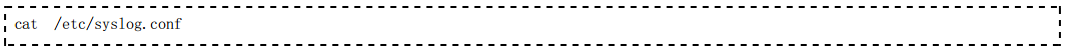
\includegraphics{catsyslog.png}

可以查看此文件的内容为:

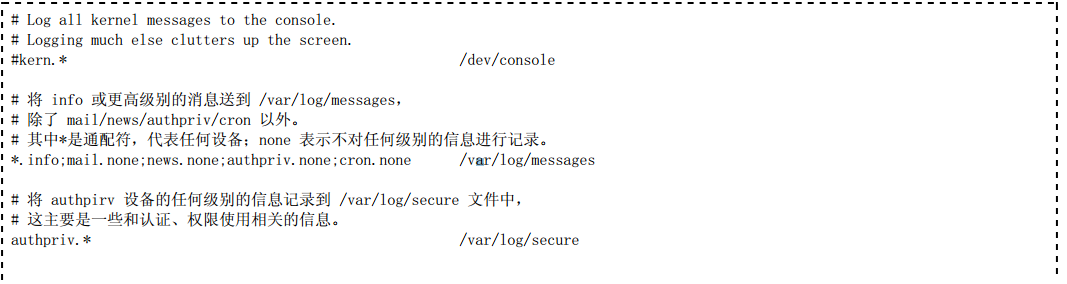
\includegraphics{syslogconf1.png}

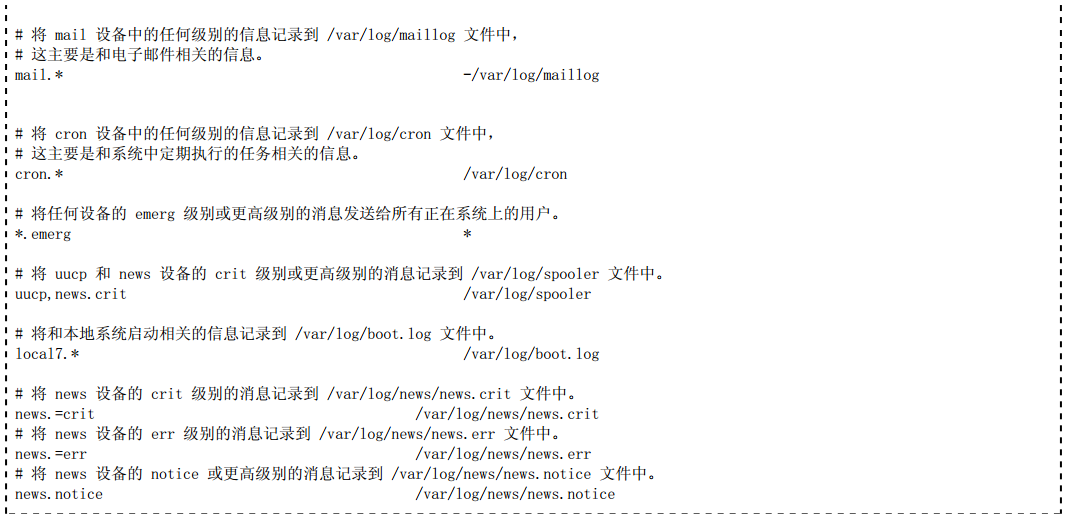
\includegraphics{syslogconf2.png}

该配置文件的每一行的格式如下:

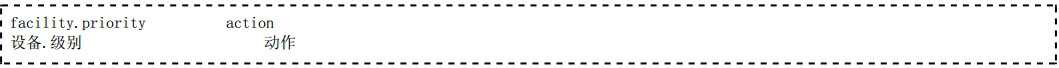
\includegraphics{format.png}

其中:

1、设备字段用来指定需要监视的事件。它可取的值如下:

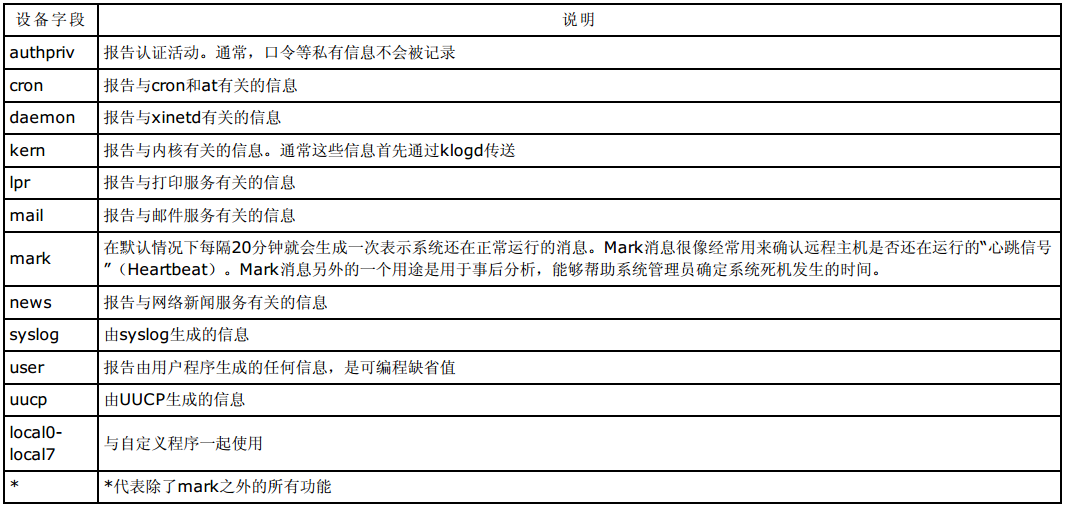
\includegraphics{faility.png}

2、级别字段用于指明与每一种功能有关的级别和优先级。它可取的值如下:


\includegraphics{prio1.png}

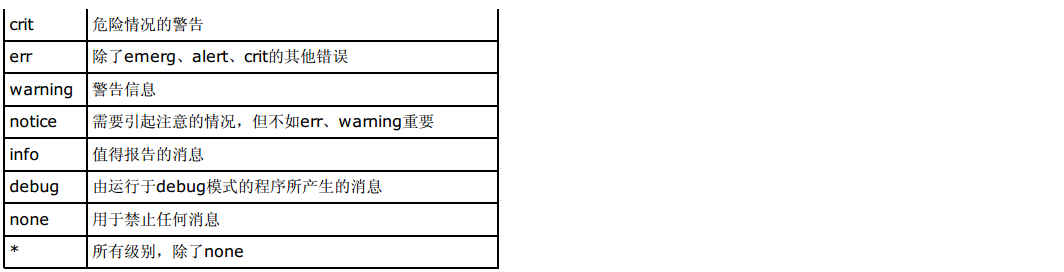
\includegraphics{prio2.png}

3、动作字段用于描述对应功能的动作。它可取的值如下:

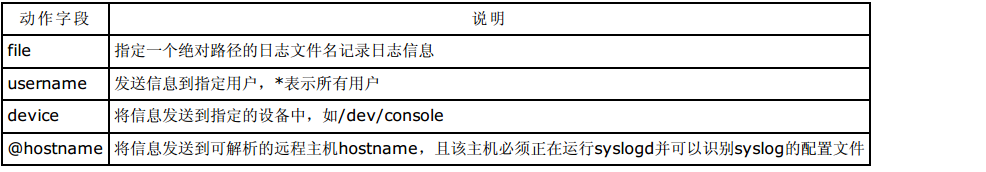
\includegraphics{action1.png}

syslog 可以为某一事件指定多个动作,也可以同时指定多个功能和级别,它们之间用分号间隔。


\subsubsection{查看日志}
\label{Linux_log/syslog:id2}
1、常见的日志文件

日志文件通常存放在 /var/log 目录下。在该目录下除了包括 syslogd 记录的日志之外,同时还包含所有应用程序的
日志。

为了查看日志文件的内容必须要有 root 权限。日志文件中的信息很重要,只能让超级用户有访问这些文件的权限。
管理员可以使用下面的命令

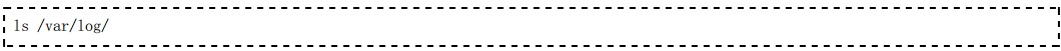
\includegraphics{lslog.png}

查看系统中使用的日志文件,常用的日志文件如表所示。

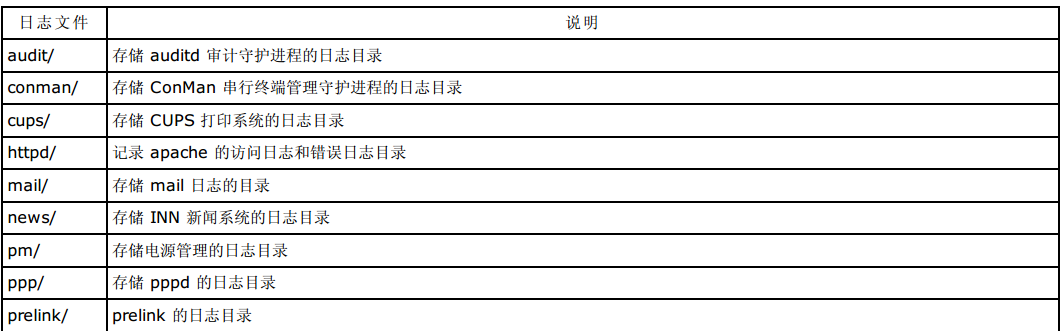
\includegraphics{log1.png}

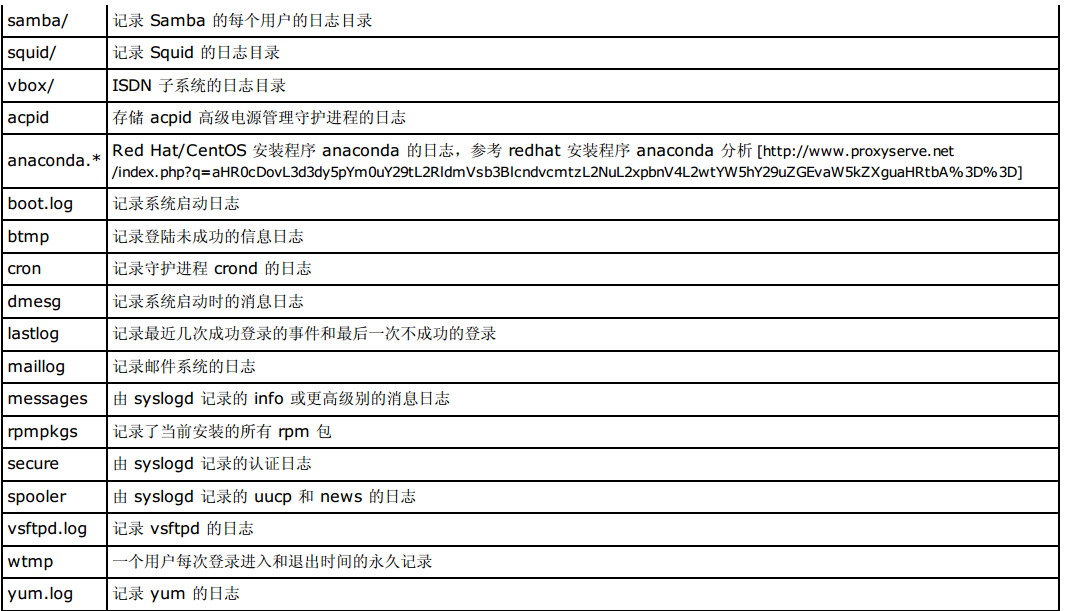
\includegraphics{log2.png}

2、查看文本日志文件

绝大多数日志文件是纯文本文件,每一行就是一个消息。只要是在Linux下能够处理纯文本的工具都能用来查看日志文
件。可以使用 cat、tac、more、less、tail 和 grep 进行查看。

下面以 /var/log/message s 为例,说明其日志文件的格式。

该文件中每一行表示一个消息,而且都由四个域的固定格式组成:

时间标签(Timestamp):表示消息发出的日期和时间。

主机名(Hostname):表示生成消息的计算机的名字。

生成消息的子系统的名字:可以是“Kernel”,表示消息来自内核或者是进程的名字,表示发出消息的程序的名字。

在方括号里的是进程的PID。

消息(Me ssage),即消息的内容。

例如:

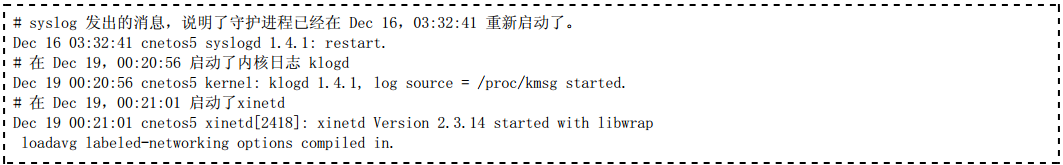
\includegraphics{message.png}

可以看出,实际上在 /var/log/message 文件中的消息都不是特别重要或紧急的。

3、查看非文本日志文件

也有一些日志文件是二进制文件,需要使用相应的命令进行读取。

1)lastlog

使用 lastlog 命令来检查某特定用户上次登录的时间,并格式化输出上次登录日志 /var/log/lastlog 的内容。例
如:

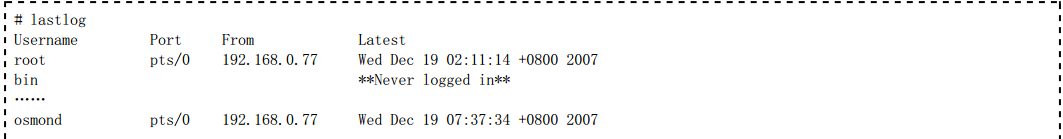
\includegraphics{lastlog.png}

2)last

last 命令往回搜索 /var/log/wtmp 来显示自从文件第一次创建以来登录过的用户。例如:

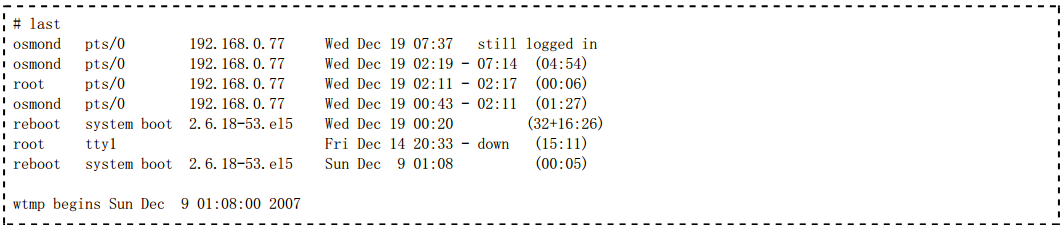
\includegraphics{last.png}

3)lastb

lastb 命令搜索 /var/log/btm p 来显示登录未成功的信息。例如:

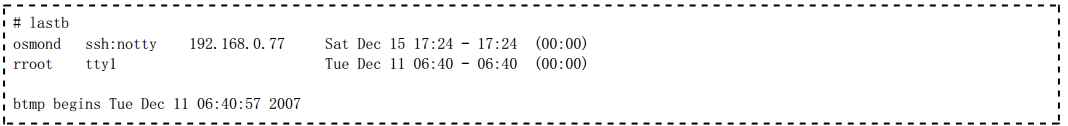
\includegraphics{lastb.png}

4)who

who 命令查询 wtm p 文件并报告当前登录的每个用户。who 命令的缺省输出包括用户名、终端类型、登录日期及远程
主机。例如:

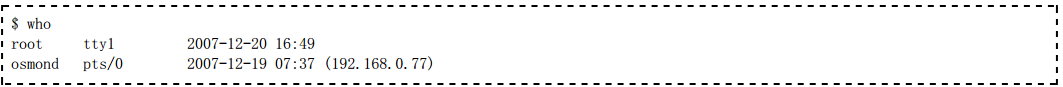
\includegraphics{who.png}

\begin{notice}{warning}{警告:}
last 与lastlog的区别
\end{notice}

last 指的是最近登录的记录,且只记录有登录记录的用户,没有登录的不记录,可能一个用户有多次登录记录,也包括正在登录的记录(正在登录的现实still login)

lastlog 记录最近一次用户登录的记录每个用户只有一条记录,切包括哪些没有登录的(显示Nerver Login )

\begin{notice}{warning}{警告:}
utmp和wtmp的区别
\end{notice}

/var/run/utmp   --  database of currently logged-in users

/var/log/wtmp  --  database of past user logins

5)其他查询命令

w命令查询utmp文件并显示当前系统中每个用户和它所运行的进程信息

ac命令根据当前的/var/log/wtmp文件中的登录进入和退出来报告用户连结的时间(小时)

users用单独的一行打印出当前登录的用户,每个显示的用户名对应一个登录会话


\subsection{日志回滚}
\label{Linux_log/logrotate::doc}\label{Linux_log/logrotate:id1}
为什么使用日志滚动

所有的日志文件都会随着时间的推移和访问次数的增加而迅速增长,因此必须对日志文件进行定期清理以免造成磁盘空
间的不必要的浪费。同时也加快了管理员查看日志所用的时间,因为打开小文件的速度比打开大文件的速度要快。

logrotate

Linux 下有一个专门的日志滚动处理程序 logrotate 能够自动完成日志的压缩、备份、删除、和日志邮寄等工作。每个日志文件都可被设置成每日,每周或每月处理,也能在文件太大时立即处理。一般把 logrota te 加入
到系统每天执行的计划任务中,这样就省得管理员自己去处理了。

其命令格式为:
\begin{description}
\item[{选项说明如下:}] \leavevmode\begin{itemize}
\item {} 
-d:详细显示指令执行过程,便于排错或了解程序执行的情况。

\item {} 
-f:强行启动记录文件维护操作,即使 logrota te 指令认为无需要亦然。

\item {} 
-m comm and:指定发送邮件的程序,默认为 /usr/bin/m ail。

\item {} 
-s sta te file:使用指定的状态文件。

\item {} 
-v:在执行日志滚动时显示详细信息。

\item {} 
-?:显示命令帮助。

\item {} 
--usage:显示使用摘要信息。

\end{itemize}

\end{description}

\textless{}configfile\textgreater{} 是 logrotate 命令的配置文件的路径。

logrotate 的配置文件

管理员可以在 logrota te 的配置文件中设置日志的滚动周期,日志的备份数目,以及如何备份日志等等。
\begin{itemize}
\item {} 
logrota te 默认的主配置文件是 /etc/logrotate.conf

\item {} 
/etc/logrotate.d 的目录下的文件,这些文件被 include 到主配置文件 /etc/logrotate.conf 中

\end{itemize}

在这些文件中可以使用如下的配置语句。

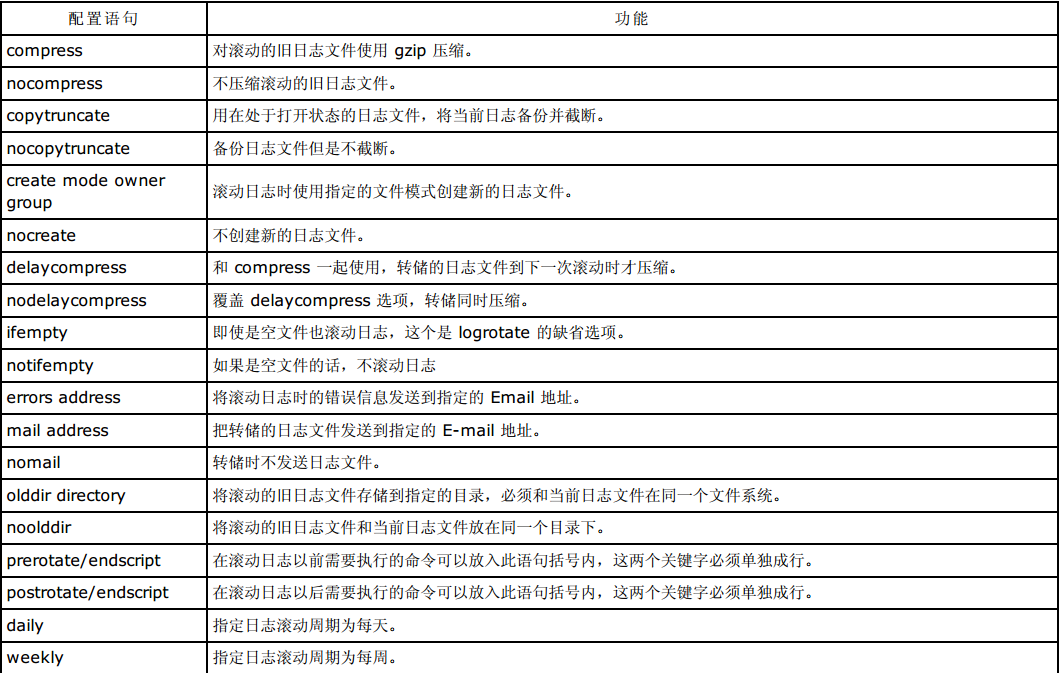
\includegraphics{logroateconfig.png}

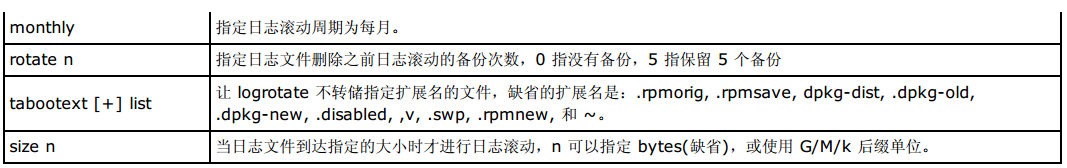
\includegraphics{logroateconfig2.png}
\begin{enumerate}
\item {} 
在 /etc/logrotate.conf 中可以使用以上的配置语句设置全局值

\end{enumerate}

2.在 /etc/logrotate.conf 中使用 include 语句包含的配置文件中也可以使用上述的配置语句,被 include 的
配置文件中的语句会覆盖 /etc/logrotate.conf 中的配置
\begin{enumerate}
\setcounter{enumi}{2}
\item {} 
为指定的文件配置日志滚动使用如下的语法

\end{enumerate}

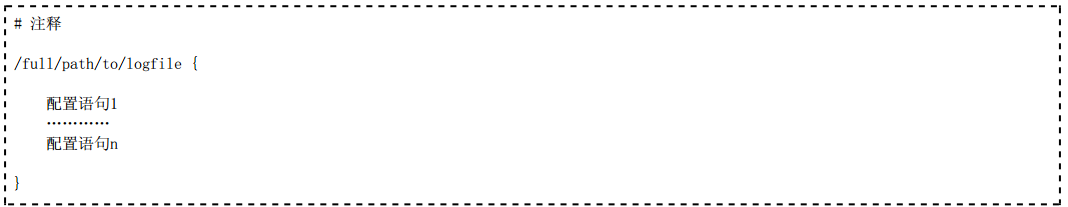
\includegraphics{file.png}


\section{Linux VIM}
\label{Linux_vim/index:linux-vim}\label{Linux_vim/index::doc}
主要内容包括vim的安装配置,常用技巧


\subsection{安装配置篇}
\label{Linux_vim/install::doc}\label{Linux_vim/install:id1}
vim的安装,vim插件的安装,语法高亮、项目视图配置


\subsubsection{vim的安装}
\label{Linux_vim/install:vim}
1、Debian 系列

apt-get install vim

2、Redhat 系列

yum install vim


\subsubsection{vim插件管理器安装}
\label{Linux_vim/install:id2}
最好也要安装vim-scripts 和vim-addon-manager 这两个是插件管理器
安装好之后,可以方便的在线进行插件的安装

1、Debian 系列

apt-get install vim-scripts vim-addon-manager

2、Redhat 系列

yum install vim-scripts vim-addon-manager

3、安装插件

vim-addons install taglist   ---安装taglist 插件


\subsubsection{vim的配置}
\label{Linux_vim/install:id3}

\paragraph{语法高亮}
\label{Linux_vim/install:id4}
vim 版本5之后就支持语法高亮显示

1、首先查看vim版本,如果符合要求则进行下一步

2、编辑vim配置文件vimrc  vim /etc/vim/vimrc,这是系统中公共的vim配置文件,对所有用户都有效
\begin{quote}

1)打开vimrc,添加以下语句来使得语法高亮显示

syntax on

2)如果此时语法还是没有高亮显示,那么在/etc目录下的profile文件中添加以下语句

export TERM=xterm-color
\end{quote}


\paragraph{项目视图}
\label{Linux_vim/install:id5}
项目试图就是这种:

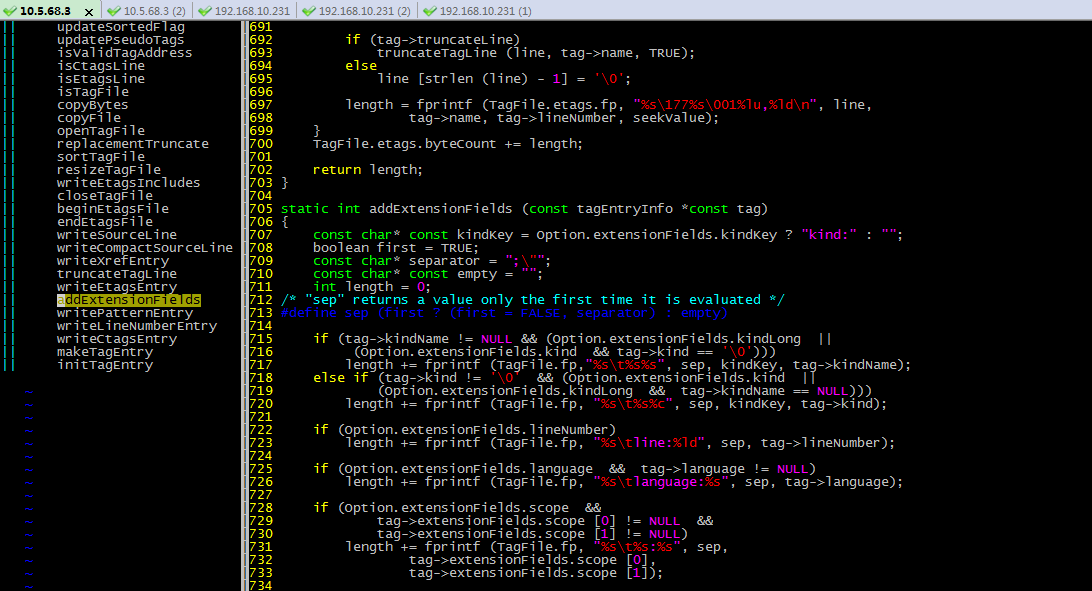
\includegraphics{view.png}

1、下载安装Exuberant Ctags

2、假设ctags 可执行文件安装于:/usr/local/bin目录下

在vimrc中加入

let Tlist\_Ctags\_Cmd='/usr/local/bin/ctags'

或者在.bashrc中加入

Export Tlist\_Ctags\_Cmd='/usr/local/bin/ctags'

3、然后用vim-add-manager下载安装Tasklist 插件

vim-addons install taglist

4、在vim normal 模式下执行命令:TlistToggle

5、退出项目试图就在normal模式下再次执行TlistToggle即可


\paragraph{语法提示和自动完成}
\label{Linux_vim/install:id6}
1、下载pythoncomplete.vim并将其放在\textless{}Vim安装目录\textgreater{}/\textless{}\$VIMRUNTIME\textgreater{}/autoload/目录下(一般为:/usr/share/vim/vim版本/autoload)

2、在vimrc中添加

filetype plugin on

set ofu=syntaxcomplet

autocmd FileType python

set omnifunc=pythoncomplete

autocmd FileType python runtime! autoload/pythoncomplete.vim

3、然后在用vim编辑python代码文件时候通过ctrl-x ctrl-o 或者 ctrl+n来打开文法提示上下文菜单,如下图所示:

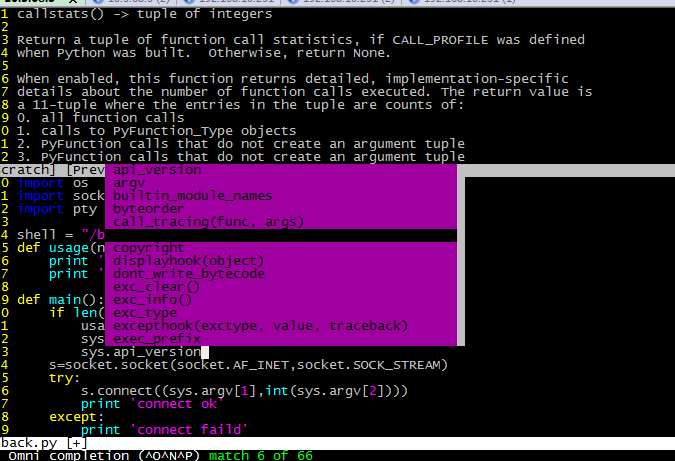
\includegraphics{menu.png}


\paragraph{FAQ}
\label{Linux_vim/install:faq}
1、vim 的配置文件默认在什么位置

vim启动的时候会读取配置文件,配置文件一般位置为:/etc/vim/vimrc

/etc/vim/gvimrc   ---适用于Gui VIM

另外还有一个配置文件:/usr/share/vim/vim73/debian.vim

这个配置文件不建议直接修改,而是修改vimrc,因为vimrc中的配置文件会直接覆盖debian.vim 的配置

2、vim 插件的位置
\begin{quote}

2.1 语法类的插件一般位置为:

/usr/share/vim/vim73/syntax (作用:用于识别不同类型语言的代码文件,为语法高亮显示提供支持)

(如果vim不能自动识别语法文件,还需要在vim中执行命令:set filetype=language,如:set filetype=python。)

2.2 标准插件的位置:

/usr/share/vim/vim73/plugin ,vim每次启动的时候都会加载这个文件夹内的文件

2.3编译类的插件位置:

/usr/share/vim/vim73/compiler顾名思义就是为能够在Vim直接编译某些语言编写的程序提供支持,其他的插件也都位于

/usr/share/vim/vim73 目录下的相应目录
\end{quote}

3.vimrc配置文件中常用的设置

set nocompatible '' explictly get out of vi-compatible mode

set background=dark '' we plan to use a dark background

syntax on  '' syntax highlighting on

set number  '' turn on line numbers

set ruler  ``always show current position along the bottom

set incsearch  '' do highlight as you type you search phrase

set ignorecase  '' case insensitive by default

set smartcase  '' if there are caps, go case-sensitive

colorscheme macvim '' the color scheme I am using now

'' 1 tab == 4 spaces

set shiftwidth=4

set tabstop=4

'' Enable filetype plugins

filetype on

filetype plugin on

filetype indent on

``设置python 自动补充

set ofu=syntaxcomplet

autocmd FileType python

set omnifunc=pythoncomplete

autocmd FileType python runtime! autoload/pythoncomplete.vim

'' Set utf8 as standard encoding and en\_US as the standard language

set encoding=utf8

set langmenu=zh\_CN.UTF-8

``设置缩进

set autoindent '' same level indent

set smartindent '' next level indent

set expandtab

set tabstop=4

set shiftwidth=4

set softtabstop=4


\subsection{系统篇}
\label{Linux_vim/command::doc}\label{Linux_vim/command:id1}

\subsubsection{Vi简介}
\label{Linux_vim/command:vi}
Vi 是 “Visual interface” 的简称,它可以执行输出、删除、查找、替换、块操作等众多文本操作,而且用户可以根据自己的需要对其进行定制,这是其他编辑程序所没有的。

Vi 不是一个排版程序,它不像 M\$ Word 或 WPS 那样可以对字体、格式、段落等其他属性进行编排,它只是一个文本编辑程序。

Vi 是全屏幕文本编辑器,它没有菜单,只有命令。


\subsubsection{进入Vi}
\label{Linux_vim/command:id2}
在命令行下键入 vi 即可进入 Vi 界面。还有如下几种进入方法:

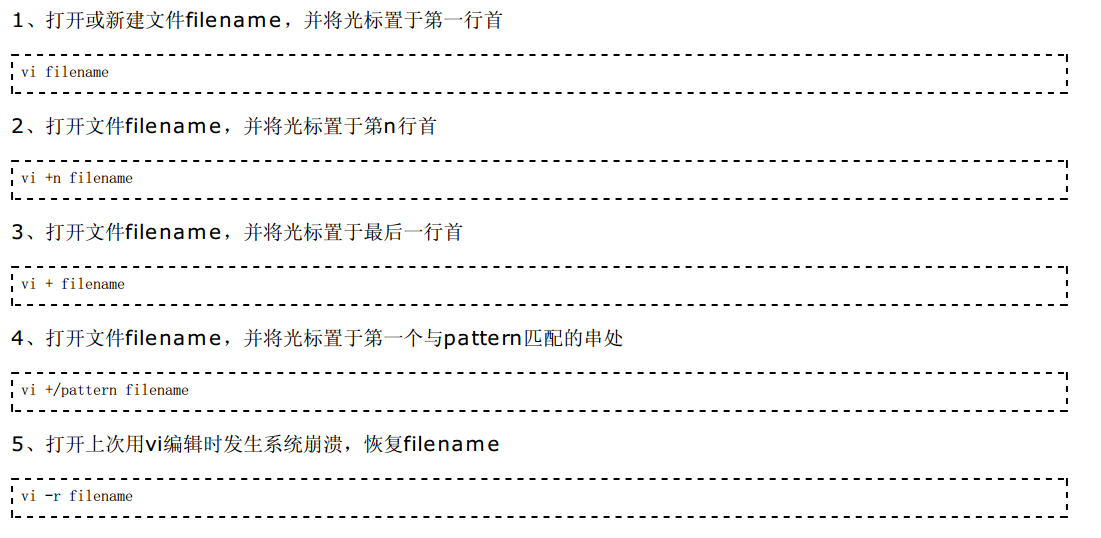
\includegraphics{vi.png}


\subsubsection{Vi 的3种运行模式}
\label{Linux_vim/command:vi-3}
Vi 有3种基本工作模式:普通(norm al)模式、插入(insert)模式和命令行(comm and-line 或 Cm dline)模式。

进入Vi之后,首先进入的就是普通模式,进入普通模式后Vi等待编辑命令输入而不是文本输入,也就是说这时输入的字
母都将作为命令来解释。在普通 (norm al) 模式里,你可以输入所有的普通编辑命令。普通模式亦称为命令
(comm and) 模式。

进入普通模式后光标停在屏幕第一行首位上(用\_表示),其余各行的行首均有一个“\textasciitilde{}”符号,表示该行为空行。最后一
行是状态行,显示出当前正在编辑的文件名及其状态。如果是[New File],则表示该文件是一个新建的文件。如果输
入Vi带文件名后,文件已在系统中存在,则在屏幕上显示出该文件的内容,并且光标停在第一行的首位,在状态行显示
出该文件的文件名、行数和字符数

在普通模式下输入插入命令i、附加命令a、打开命令o、修改命令c、取代命令r或替换命令s都可以进入插入模式。在插
入模式下,用户输入的任何字符都被Vi当作文件内容保存起来,并将其显示在屏幕上。在文本输入过程中,若想回到命
令行模式下,按Esc键即可。

在普通模式下,执行 Ex 命令使用 :,查找使用 ? 和 /,调用过滤命令使用 !。多数文件管理命令都是在此模式下执行
的。末行命令执行完后,Vi自动回到普通模式。

关于这3种模式的转换如图所示。

Vi 三种模式之间的转换示意图


\paragraph{普通模式下的操作}
\label{Linux_vim/command:id3}
1.进入插入模式

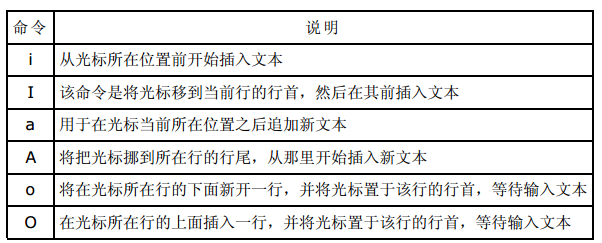
\includegraphics{insert.png}

2、光标定位

\includegraphics{Location.png}

3、替换和删除

\includegraphics{replace.png}

4、复制和粘贴

\includegraphics{copy.png}

5、搜索字符串

\includegraphics{search.png}

6、撤销和重复

\includegraphics{repeat.png}

7、退出 Vi

\includegraphics{exit.png}


\paragraph{命令行模式下的操作}
\label{Linux_vim/command:id4}
1、跳行

\includegraphics{jump.png}

2、字符串搜索、替换

\includegraphics{str_search.png}

vi 支持基本的正则表达式 Basic regular expre ssion (BRE),上述命令中的 str 和 str1 可以使用正则表达式进
行搜索。

3、文本的复制、移动和删除

\includegraphics{text_cp.png}

4、文件相关

\includegraphics{file1.png}

5、执行 Shell 命令

\includegraphics{shell.png}

6、设置 Vi 环境

\includegraphics{setvi.png}

7、退出 Vi

\includegraphics{exitvi.png}


\subsection{技巧篇}
\label{Linux_vim/tips::doc}\label{Linux_vim/tips:id1}
vim 常用技巧,值得去看


\subsubsection{常用技巧}
\label{Linux_vim/tips:id2}
1、如何去掉vim打开的文件中的\textasciicircum{}M
\begin{quote}

:\%s/r/
\begin{quote}

其他可以参考的方法

tr -d ``\textbackslash{}r'' \textless{} src \textgreater{}dest

tr -d ``\textbackslash{}015'' dest
\end{quote}

cat filename1 \textbar{} tr -d ``\textasciicircum{}V\textasciicircum{}M'' \textgreater{} newfile;

sed -e ``s/\textasciicircum{}V\textasciicircum{}M//'' filename \textgreater{}

:\%s/\textasciicircum{}M\$//g
\begin{quote}

strings A\textgreater{}B
\end{quote}

(windows rn  0d0a;linux n 0a)
\end{quote}

2、vim 跨文件复制
\begin{quote}

1)用vim打开一个文件,例如:original.trace

2)在普通模式下,输入:'':sp''(不含引号)横向切分一个窗口,或者'':vsp''纵向切分一个窗口,敲入命令后,你将看到两个窗口打开的是同一个文件

3)在普通模式下,输入:'':e new.trace'',在其中一个窗口里打开另一个文件

4)切换到含有源文件(original.trace)的窗口,在普通模式下,把光标移到你需要复制内容的起始行,然后输入你想复制的行的数量(从光标所在行往下计算),在行数后面接着输入yy,这样就将内容复制到临时寄存器里 了(在 普通模式下ctrl+w,再按一下w,可以在两个窗口之间切换)

5)切换到目标文件(new.trace)窗口,把光标移到你接收复制内容的起始行,按一下p,就完成复制了。
\end{quote}

3、3、修改文件的编码
\begin{quote}

1)查看当前vim打开文件内容的编码

:set fileencoding

2)设置新编码

:set fileencoding=utf-8
\end{quote}

4、连续删除1,到n行
\begin{quote}

:1,10d
\end{quote}

5、vim连续注释多行
\begin{quote}

:1,10s/\textasciicircum{}/\#/g
\end{quote}

6、取消连续多行的注释
\begin{quote}

:1,10s/\#/\textasciicircum{}/g
\end{quote}

7、多行整体向右移动若干个tab
\begin{quote}

:1,10\textgreater{}\textgreater{}
\end{quote}

8、多行整体向←移动若干个tab
\begin{quote}

:1,10\textless{}\textless{}
\end{quote}

9、vim 插入的命令
\begin{quote}

a       在光标之后插入

i       在光标之前插入

o       在下行插入

O       在上行插入
\end{quote}

10、定位到第一行
\begin{quote}

gg

:1
\end{quote}

11、定位到最后一行
\begin{quote}

G

:\$
\end{quote}
\begin{description}
\item[{12、删除文件所有内容}] \leavevmode
:\%d

\end{description}

13、无插件Vim编程技巧
\begin{quote}

\href{http://coolshell.cn/articles/11312.html}{http://coolshell.cn/articles/11312.html}
\end{quote}

14、vim 替换

vi/vim 中可以使用 :s 命令来替换字符串。该命令有很多种不同细节使用方法,可以实现复杂的功能

:s/vivian/sky/ 替换当前行第一个 vivian 为 sky

:s/vivian/sky/g 替换当前行所有 vivian 为 sky

:n,\$s/vivian/sky/ 替换第 n 行开始到最后一行中每一行的第一个 vivian 为 sky

:n,\$s/vivian/sky/g 替换第 n 行开始到最后一行中每一行所有 vivian 为 sky

:s\#vivian/\#sky/\# 替换当前行第一个 vivian/ 为 sky/

:\%s+/oradata/apras/+/user01/apras1+ (使用+ 来 替换 / ): /oradata/apras/替换成/user01/apras1/

:s/vivian/sky/ 替换当前行第一个 vivian 为 sky

:s/vivian/sky/g 替换当前行所有 vivian 为 sky

:\%s/vivian/sky/ 替换每一行的第一个 vivian 为 sky

:\%s/vivian/sky/g  替换每一行中所有 vivian 为 sky

s/vivian/sky/gc  替换当前行所有 vivian 为 sky ,在替换之前进行替换确认,c是confirm的缩写


\section{大话SSH}
\label{Linux_ssh/index::doc}\label{Linux_ssh/index:ssh}
你需要掌握的

1、ssh安全配置

2、ssh 隧道

3、ssl 端口转发


\subsection{ssh 安全配置}
\label{Linux_ssh/config::doc}\label{Linux_ssh/config:ssh}
\textbf{1、sshd\_confg 安全配置}

1)禁止root 登录

2)禁止空口令登录

3)禁止kndown host 登录

4)禁止端口转发

5)使用1024位公钥(默认是768)

6)只允许指定用户\textbar{}用户组登录

\textbf{2、ssh登录限制配置思路}

1)使用tcpwrapper

你可在 hosts.allow 中设:

sshd: 192.168.0.1

sshd: ALL: deny

只允许192.168.0.1 主机登录

2)iptables

iptables -I INPUT -p tcp --dport 22 -j DROP

iptables -I INPUT -p tcp --dport 22 -s 192.168.0.0/32 -j ACCEPT

(注:用 -I 命令,且顺序不能颠倒...)

3)使用pam模块
\begin{quote}

修改 /etc/pam.d/sshd

auth required pam\_listfile.so item=user sense=allow file=/etc/sshusers onerr=fail

将你要的用户写进/etc/sshusers ,如:

echo ``zhangsan'' \textgreater{}\textgreater{} /etc/sshusers

设定登录黑名单

vi /etc/pam.d/sshd

增加

auth required /lib/security/pam\_listfile.so item=user sense=deny file=/etc/sshd\_user\_deny\_list onerr=succeed

所有/etc/sshd\_user\_deny\_list里面的用户被拒绝ssh登录
\end{quote}

4)使用sshd\_config配置文件

允许或者禁止某个用户(组)通过ssh登录

在/etc/ssh/sshd\_conf添加

AllowUsers 用户名

或者

AllowGroups 组名

或者

DenyUsers 用户名

\textbf{3、ssh 暴力破解防护}

1)限制IP

iptables、tcpwraper都可以做

2)限制用户(组)
\begin{quote}

sshd可做

pam(黑名单、白名单)
\end{quote}

3)只允许公钥登录

4)指定尝试密码次数

vi /etc/sshd\_config

修必MaxAuthTries 3

\textbf{4、ssh 中间人攻击原理与防护}

1)原理

dh算法是这样的,A和B先共享p,q。然后A生成随机数a,计算E1=(p\textasciicircum{}a)modq发给B,B生成随机数b,计算E2=(p\textasciicircum{}b)modq发给A;A计算K=E2\textasciicircum{}a=(p\textasciicircum{}ab)modq,B计算K=E1\textasciicircum{}b=(p\textasciicircum{}ba)modq,就共享了K这个密钥吧,

C假设是中间人,他知道E1和E2,p,q

他也生成一个随机数c,计算Ec=(p\textasciicircum{}c)modq给A和B

这个时候E1,E2被截获没有发给对方,都在中间被C拦截住了

A收到Ec以为是E2,B收到Ec以为是E1

A计算Kac=Ec\textasciicircum{}a=p\textasciicircum{}ca,B计算Kbc=Ec\textasciicircum{}b=p\textasciicircum{}cb

C就可以中间人了

E1、E2、p、q这些信息全部用服务器公钥加密传输

2)防护

注意server端公钥指纹的变化

\textbf{5、公钥自动登录设置}

ssh-keygen 和ssh-copy-id实现ssh自动登录

本实验的前提是:两者都是linux系统,且一端是ssh-server(192.168.11.164),一端是ssh-client(192.168.11.103)

在ssh-client执行如下操作

1)ssh-keygen -t rsa   ===\textgreater{}这条命令用来生成rsa密钥对(一个公钥,一个私钥,.pub结尾的是公钥,这里-t的参数就是指定使用的算法,主要有三种 rsa dsa 用于ssh2 ,rsa1用于ssh1,这里以ssh2为例实验)

在ssh-client当前用户的家目录下面的.ssh目录下面会出现两个文件id\_rsa id\_rsa.pub

2)ssh-copy-id -i id\_rsa.pub \href{mailto:root@192.168.11.164}{root@192.168.11.164}

出现如下:

\href{mailto:root@192.168.11.164's}{root@192.168.11.164's} password:

Now try logging into the machine, with ``ssh \href{mailto:'root@192.168.11.164}{`root@192.168.11.164}`'', and check in:
\begin{quote}

.ssh/authorized\_keys
\end{quote}

to make sure we haven't added extra keys that you weren't expecting.

这样当你在当前的ssh-client用户环境中去以root身份登录192.168.11.164这台机器的时候,会不用输入密码而自动登录的

当你登录到192.168.11.164这台机器后,你会发现在root会用的\textasciitilde{}/.ssh目录下面有一个名为authorized\_keys的文件,这个文件存储有ssh-client发送的公钥信息

当然你也可以选择以不同用户身份自动登录进入ssh-server,只要将对应的公钥信息拷贝至相应的用户的.ssh/authorized\_keys文件中即可

3、ssh-copy-id应注意的小地方

Default public key: ssh-copy-id uses \textasciitilde{}/.ssh/identity.pub as the default public key file (i.e when no value is passed to option -i). Instead, I wish it uses id\_dsa.pub, or id\_rsa.pub, or identity.pub as default keys. i.e If any one of them exist, it should copy that to the remote-host. If two or three of them exist, it should copy identity.pub as default.
The agent has no identities: When the ssh-agent is running and the ssh-add -L returns “The agent has no identities” (i.e no keys are added to the ssh-agent), the ssh-copy-id will still copy the message “The agent has no identities” to the remote-host’s authorized\_keys entry.
Duplicate entry in authorized\_keys: I wish ssh-copy-id validates duplicate entry on the remote-host’s authorized\_keys. If you execute ssh-copy-id multiple times on the local-host, it will keep appending the same key on the remote-host’s authorized\_keys file without checking for duplicates. Even with duplicate entries everything works as expected. But, I would like to have my authorized\_keys file clutter free.


\section{Linux 进程管理}
\label{Linux_pro_mana/index::doc}\label{Linux_pro_mana/index:linux}
主要内容包括:后台进程、任务、进程查看工具使用、性能工具使用


\subsection{进程与作业}
\label{Linux_pro_mana/process::doc}\label{Linux_pro_mana/process:id1}\begin{enumerate}
\item {} 
掌握进程的相关概念

\item {} 
熟悉Linux中进程的类型和启动方式

\item {} 
学会查看和杀死进程

\item {} 
理解何谓作业控制

\item {} 
掌握实施作业控制的常用命令

\end{enumerate}


\subsubsection{进程概述}
\label{Linux_pro_mana/process:id2}

\paragraph{进程的概念}
\label{Linux_pro_mana/process:id3}
进程(Proce ss)是一个程序在其自身的虚拟地址空间中的一次执行活动。之所以要创建进程,就是为了使多个程序可
以并发的执行,从而提高系统的资源利用率和吞吐量。

进程和程序的概念不同,下面是对这两个概念的比较
\begin{itemize}
\item {} 
程序只是一个静态的指令集合;而进程是一个程序的动态执行过程,它具有生命期,是动态的产生和消亡的。

\item {} 
进程是资源申请、调度和独立运行的单位,因此,它使用系统中的运行资源;而程序不能申请系统资源、不能被系统调度、也不能作为独立运行的单位,因此,它不占用系统的运行资源。

\item {} 
程序和进程无一一对应的关系。一方面一个程序可以由多个进程所共用,即一个程序在运行过程中可以产生多个进程;另一方面,一个进程在生命期内可以顺序的执行若干个程序。

\end{itemize}

Linux操作系统是多任务的,如果一个应用程序需要几个进程并发地协调运行来完成相关工作,系统会安排这些进程并
发运行,同时完成对这些进程的调度和管理任务,包括CPU、内存、存储器等系统资源的分配。


\paragraph{Linux中的进程}
\label{Linux_pro_mana/process:linux}
在Linux系统中总是有很多进程同时在运行,每一个进程都有一个识别号,叫做PID(Proce ss ID),用以区分不同
的进程。系统启动后的第一个进程是init,它的PID是1。init是唯一一个由系统内核直接运行的进程。新的进程可以用
系统调用fork来产生,就是从一个已经存在的旧进程中分出一个新进程来,旧的进程是新产生的进程的父进程,新进程
是产生它的进程的子进程,除了init之外,每一个进程都有父进程。当系统启动以后,init进程会创建login进程等待用
户登录系统,login进程是init进程的子进程。当用户登录系统后,login进程就会为用户启动shell进程,shell进程就
是login进程的子进程,而此后用户运行的进程都是由shell衍生出来的。

init进程是所有进程的发起者和控制者。因为在任何基于Unix的系统(比如linux)中,它都是第一个运行的进程,所以init进程的编号(ProcessID,PID)永远是1。
如果init 出现了问题,系统的其余部分也就随之而垮掉了。

init进程有两个作用。
\begin{itemize}
\item {} 
第一个作用是扮演终结父进程的角色。因为init进程永远不会被终止,所以系统总是可以确信它的存在,并在必要的时候以它为参照。如果某个进程在它衍生出来的全部子进程结束之前被终止,就会出现必须以init 为参照的情况。此时那些失去了父进程的子进程就都会以init作为它们的父进程。快速执行一下ps-af 命令,可以列出许多父进程ID(ParentProcessID,PPID)为1的进程来。

\item {} 
init 的第二个角色是在进入某个特定的运行级别(Runlevel)时运行相应的程序,以此对各种运行级别进行管理。它的这个作用是由/etc/inittab文件定义的

\end{itemize}

除了进程识别号外,每个进程还有另外四个识别号。它们是实际用户识别号(real user ID)、实际组识别号以及有效
用户识别号(e ffe ct user ID),和有效组识别号(e ffe ct group ID)。实际用户识别号和实际组识别号的作用是
识别正在运行此进程的用户和组。一个进程的实际用户识别号和实际组识别号就是运行此进程的用户的识别号(UID)
和组的识别号(GID)。有效用户识别号和有效组识别号的作用是确定一个进程对其访问的文件的权限和优先权。除了
产生进程的程序被设置UID位和GID位之外,一般有效用户识别号和有效组识别号和实际用户识别号及实际组识别号相
同。如果程序被设置了UID位或GID位,则此进程相应的有效用户识别号和有效组识别号,将和运行此进程的文件的所
属用户的UID或所属组的GID相同。

例如,一个可执行文件/usr/bin/passwd,其所属用户是root(UID为0),此文件被设置了UID位。则当一个UID为500、GID为501的用户执行此命令时,
产生的进程的实际用户识别号和实际组识别号分别是500和501,而其有效用户识别号是0,有效组识别号是501。

所有这些设计都是为了在一个多用户、多任务的操作系统中,所有用户的工作都能够安全可靠地进行,这也是Linux操
作系统的优秀性所在。


\paragraph{进程的类型}
\label{Linux_pro_mana/process:id4}
可以将运行在Linux系统中的进程分为三种不同的类型:
\begin{itemize}
\item {} 
交互进程:由一个Shell启动的进程。交互进程既可以在前台运行,也可以在后台运行。

\item {} 
批处理进程:不与特定的终端相关联,提交到等待队列种顺序执行的进程。

\item {} 
守护进程:在Linux在启动时初始化,需要时运行于后台的进程。

\end{itemize}

以上三种进程各有各的特点、作用和不同的使用场合。


\paragraph{进程的启动方式}
\label{Linux_pro_mana/process:id5}
启动一个进程有两个主要途径∶手工启动和调度启动。

1、手工启动:由用户输入命令,直接启动一个进程便是手工启动进程。手工启动进程又可以分为前台启动和后台启动。
\begin{quote}

I .前台启动:是手工启动一个进程的最常用的方式。一般地,用户键入一个命令“ls -l”,这就已经启动了一个进程,而且是一个前台的进程。

II.后台启动:直接从后台手工启动一个进程用得比较少一些,除非是该进程甚为耗时,且用户也不急着需要结果的时候。假设用户要启动一个需要长时间运行的格式化文本文件的进程。为了不使整个shell在耗时进程的运行过程中都处于“瘫痪”状态,从后台启动这个进程是明智的选择。在后台启动一个进程,可以在命令行后使用\&命令,例如: \# ls –R / \textgreater{}list \&
\end{quote}

2、调度启动方式是事先进行设置,根据用户要求让系统自行启动。如安排周期性任务


\paragraph{进程的属性}
\label{Linux_pro_mana/process:id6}
进程 ID(PID):是唯一的数值,用来区分进程;

父进程和父进程的 ID(PPID);

启动进程的用户 ID(UID)和所归属的组(GID);

进程状态:状态分为运行 R、休眠 S、僵尸 Z;

进程执行的优先级;

进程所连接的终端名;

进程资源占用:比如占用资源大小(内存、CPU 占用量);


\paragraph{进程优先级}
\label{Linux_pro_mana/process:id7}
进程优先级的范围:-19\textasciitilde{}20

系统第一个进程是init ,由内核启动,后续的所有进程都是她的子进程

一般用户的nice值是0~19

?root用户可用的nice值是-20~19

PRI是系统动态决定的,虽然 nice值可以影响PRI,但是最终的PRI还是要经过系统分析后才能决定。

nice 值可以被改变……

?在启动进程时:

\$ nice -n 5 command

?在启动后:

\$ renice 5 PID

只有根用户才能降低nice值(提高优先性)


\paragraph{linux上进程有5种状态}
\label{Linux_pro_mana/process:linux5}\begin{enumerate}
\item {} 
运行(正在运行或在运行队列中等待)

\item {} 
中断(休眠中, 受阻, 在等待某个条件的形成或接受到信号)

\item {} 
不可中断(收到信号不唤醒和不可运行, 进程必须等待直到有中断发生)

\item {} 
僵死(进程已终止, 但进程描述符存在, 直到父进程调用wait4()系统调用后释放)

\item {} 
停止(进程收到SIGSTOP, SIGSTP, SIGTIN, SIGTOU信号后停止运行运行)

\end{enumerate}


\paragraph{父进程和子进程}
\label{Linux_pro_mana/process:id8}
他们的关系是管理和被管理的关系,当父进程终止时,子进程也随之而终止。但子进程终止 ,
父进程并不一定终止。比如 httpd 服务器运行时,我们可以杀掉其子进程,父进程并不会因
为子进程的终止而终止。


\paragraph{守护进程简介}
\label{Linux_pro_mana/process:id9}
内容提要
\begin{enumerate}
\item {} 
守护进程的概念

\item {} 
超级服务器的引入

\item {} 
熟悉常见的守护进程

\end{enumerate}


\subparagraph{什么是守护进程}
\label{Linux_pro_mana/process:id10}
Linux 系统在启动时就启动很多进程(例如:init 进程、等待用户登录的进程 login、等待 FTP 客户连接的 vsftpd 等),这
些进程向本地和网络用户提供了 Linux 的系统功能接口,直接面向应用程序和用户。将这些进程称为守护进程(daem on)。
守护进程是指在后台运行而又没有终端或登录 shell 与之结合在一起的进程。由于此类程序运行在后台,除非程序异常终止或者人
为终止,否则它们将一直运行下去直至系统关闭。一般地,守护进程在系统引导装入时启动,在系统关闭时终止。一个实际运行中
的系统一般会有多个这样的守护进程在运行。Windows 系统中的守护进程被称为“服务”。

按照服务类型可以分为如下两类:
\begin{itemize}
\item {} 
系统守护进程:如 a td、cron、lpd、syslogd、login 等。

\item {} 
网络守护进程:如 sshd、httpd、sendm ail、xine td 等。

\end{itemize}


\subparagraph{网络守护进程}
\label{Linux_pro_mana/process:id11}
在 Client/Server 模型中,服务器监听(Listen)在一个特定的端口上等待客户的连接。连接成功之后客户机与服务器通过端口
进行数据通讯。

守护进程的工作就是打开一个端口,并且等待(Listen)进入的连接。如果客户提请了一个连接,守护进程就创建(fork)子进
程来响应此连接,而父进程继续监听更多的服务请求。正因为如此,每个守护进程都可以处理多个客户服务请求。


\subparagraph{超级守护进程}
\label{Linux_pro_mana/process:id12}
运行 Linux 的计算机一般都作为服务器使用,提供了许多不同协议的服务。但是,一台繁忙的服务器也可能是专用于某个任务
的,比如传输邮件、响应 DNS 请求等。

从守护进程的概念,我们可以看出,对于系统所要提供的每一种服务,都必须运行一个监听某个端口连接发生的守护程序。无论如
何,在提供多种服务的 Linux 系统中,系统内存中同时运行二、三十种不同的守护进程是对资源的浪费。解决这个问题的方法是
使用超级服务器 (SuperServer)。

几乎所有的类 UNIX 系统都运行了一个“超级服务器”,它为众多服务创建套接字(Socke t),并且使用 Socke t 系统调用同时
监听多个端口。当远程系统请求一个服务时,超级服务器监听到这个请求后会产生该端口的服务器程序为客户提供服务。
使用最广泛的超级服务器程序是 xinetd ,即“扩展网络守护进程”。

xinetd 在运行时读取 /etc 下文本配置文件,在文件中指出超级服务器需要监听的端口以及在数据包到达端口时需要启动的程
序。 xinetd 具有更先进的配置模式和更好的安全性。


\subparagraph{守护进程的运行方式}
\label{Linux_pro_mana/process:id13}
由于引入了超级服务器,因此守护进程有如下两种运行方式:

1、独立运行的(stand-alone)守护进程
\begin{itemize}
\item {} 
独立运行的守护进程由 init 脚本负责管理

\item {} 
独立运行的守护进程的脚本存放在 /e tc/init.d/ 目录下

\item {} 
所有的系统服务都是独立运行的。如:cron、syslogd 等。

\end{itemize}

2、由超级服务器(SuperServer)运行的守护进程
\begin{itemize}
\item {} 
要运行的守护进程由 ine td/xine td 启动

\item {} 
由 xine td 管理的守护进程的配置文件存放在 /e tc/xine td.d/ 目录下, 默认的 xine td 的主配置文件是/etc/xine td.conf

\item {} 
ine td/xine td 本身是独立运行的守护进程

\end{itemize}

为了节省资源,引入了超级服务器用于监控网络服务,如 telne t、talk 等。使用超级服务器启动网络服务虽然可以节省资源,但
是对于服务量很大的守护进程(如 HTTP服务、FTP服务)将影响到其他服务的运行,同时也影响所提供服务的响应速度。为此,
某些常用的知名网络服务的守护进程需要单独启动。

哪些守护进程可以使用超级服务器启动?

几乎所有的网络服务程序都可以由超级服务器来启动,而具体提供哪些服务将由 /e tc/service s 文件指出。这个文件中说明了超
级服务器可提供服务的端口号和名字。


\subparagraph{查看守护进程树}
\label{Linux_pro_mana/process:id14}
可以使用 pstree 命令查看守护进程树。例如:

\includegraphics{pstree.png}


\subparagraph{守护进程的启用和停止}
\label{Linux_pro_mana/process:id15}
1、独立运行的守护进程的启用和停止
\begin{quote}

1)/etc/init.d/server-name start\textbar{}stop\textbar{}restart\textbar{}reload

2)service server-name start\textbar{}stop\textbar{}restart\textbar{}reload
\end{quote}

2、由超级服务器运行的守护进程的启用和停止
\begin{quote}

1)修改 /etc/xine td.d/ 目录下的相关文件
\begin{itemize}
\item {} 
启用服务,使用 disable = no 选项

\item {} 
停用服务,使用 disable = yes 选项

\end{itemize}

2)重新启动超级服务器

\# /etc/init.d/xinetd restart

\# service xinetd restart
\end{quote}

3、使用 chkconfig 管理启动脚本

可以使用 chk config 命令检查、设置系统的各种服务。此命令实际上是通过操控 /etc/rc{[}0-6{]}.d 目录下的符号链
接文件对系统的各种服务进行管理。

可以使用 chk config 命令检查、设置系统的各种服务。此命令实际上是通过操控 /etc/rc{[}0-6{]}.d 目录下的符号链
接文件对系统的各种服务进行管理。

chk config 命令具有如下功能:

添加指定的新服务

清除指定的服务

显示由 chk config 管理的服务

改变服务的运行级别

检查指定服务的启动状态

chk config 命令的格式如下:
\begin{quote}

\# chkconfig --list {[}server-name{]}

\# chkconfig --add server-name

\# chkconfig --del server-name

\# chkconfig {[}--level \textless{}levels\textgreater{}{]} server-name \textless{}on\textbar{}off\textbar{}reset\textbar{}resetpriorities\textgreater{}
\end{quote}

其中:

server-name:是由 chk config 命令管理的服务的名字。

--list:显示由 chk config 管理的所有服务。

--level \textless{}levels\textgreater{}:指定某服务要在哪个运行级别中开启或关闭,\textless{}levels\textgreater{} 的范围在 0-6 之间。

--add:添加由 chk config 进行管理的指定服务。

--del:删除由 chk config 进行管理的指定服务。

on\textbar{}off:在指定的运行级别,开启或关闭服务。不指定运行级别时,默认的运行级别是 3、4、5。

reset:在指定的运行级别,重置该服务,使其状态返回到操作系统启动时的默认状态。

例如:

1)查看指定的服务在所有运行级别的运行状态。
\begin{quote}

\# chkconfig --list sendmail
\end{quote}

)显示由 chk config 管理的所有服务。
\begin{quote}

\# chkconfig --list
\end{quote}

3)添加一个由chk config管理的服务。
\begin{quote}

\# chkconfig --add httpd
\end{quote}

4)更改指定服务在指定运行级别的运行状态。
\begin{quote}

\# chkconfig --level 35 httpd on

\# chkconfig httpd on

\# chkconfig --level 4 sendmail off
\end{quote}

5)启动或停用由 xine td 运行的服务
\begin{quote}

\# chkconfig rsync on \# 相当于配置文件中的 ``disable = no''

\# chkconfig rsync off \# 相当于配置文件中的 ``disable = yes''
\end{quote}


\subparagraph{管理开机时守护进程的的启用状态}
\label{Linux_pro_mana/process:id16}
若要管理守护进程在计算机启动过程中是否启动,Redhat系列操作系统可以使用 ntsysv。

执行如下命令运行 ntsysv:
\begin{quote}

\# ntsysv
\end{quote}

\includegraphics{ntsysv.png}

使用 ntsysv 管理开机时守护进程的的启用状态

可以使用上下方向键移动光标选择操作对象,使用空格键激活或终止服务({[}*{]}表示激活;{[} {]}表示终止)。操作结束单
击“确定”按钮结束(也可以单击“取消”按钮取消操作)。这样在下次启动机器时,修改将生效。

Debian系列操作系统可以使用sysv-rc-conf

\#sysv-rc-conf

\includegraphics{sysv-rc-conf.png}


\subsubsection{作业控制}
\label{Linux_pro_mana/process:id17}

\paragraph{什么是作业控制}
\label{Linux_pro_mana/process:id18}
作业控制是指控制当前正在运行的进程的行为,也称为进程控制。作业控制是Shell的一个特性,使用户能在多个独立进
程间进行切换。例如,用户可以挂起一个正在运行的进程,稍后再恢复它的运行。bash记录所有启动的进程并保持对所
有已启动的进程的跟踪,在每一个正在运行的进程的生命期内的任何时候,用户可以任意地挂起进程或重新启动进程恢
复运行。

例如,当用户使用Vi编辑一个文本文件,并需要中止编辑做其他事情时,利用作业控制,用户可以让编辑器暂时挂起,
返回Shell提示符开始做其他的事情。其他事情做完以后,用户可以重新启动挂起的编辑器,返回到刚才中止的地方,就
像用户从来没有离开编辑器一样。这只是一个例子,作业控制还有许多其他实际的用途。


\paragraph{实施作业控制的常用命令}
\label{Linux_pro_mana/process:id19}
下表列出了作业控制的常用命令或操作快捷键。

\includegraphics{job1.png}

这些命令经常用于用户需要在后台运行,而却意外地把它放到了前台启动运行的时候。当一个命令在前台被启动运行
时,它会禁止用户与Shell的交互,直到该命令结束。由于大多数命令的执行都能很快完成,所以一般情况下不会有什么
问题。但是如果要运行的命令要花费很长时间的话,我们通常会把它放到后台,以便能在前台继续输入其他命令。此
时,上面的命令就会派上用场了。

在进行作业控制时经常使用如下的作业标识符:

\includegraphics{job2.png}


\paragraph{作业控制举例}
\label{Linux_pro_mana/process:id20}
下面举一个简单的例子说明作业控制命令的使用。
\begin{quote}

\# 列出所有正在运行的作业

\$ jobs

\# 在前台运行睡眠进程

\$ sleep 100000

\# 使用Ctrl+z挂起

{[}1{]}+ Stopped sleep 100000

\# 在前台运行睡眠进程

\$ sleep 200000

\# 使用Ctrl+z挂起

{[}2{]}+ Stopped sleep 200000

\# 在后台运行睡眠进程

\$ sleep 300000 \&

{[}3{]} 8941

\# 运行cat命令

\$ cat \textgreater{}example

This is a example.

\# 使用Ctrl+z挂起

{[}4{]}+ Stopped cat \textgreater{}example

\# 列出所有正在运行的作业

\# 第1列是作业号,第2列中的+表示默认作业;-表示第二默认作业,第3列是作业状态

\$ jobs

{[}1{]} Stopped sleep 100000

{[}2{]}- Stopped sleep 200000

{[}3{]} Running sleep 300000 \&

{[}4{]}+ Stopped cat \textgreater{}example

\# 列出所有正在运行的作业,同时列出进程PID

\$ jobs -l

{[}1{]} 8939 Stopped sleep 100000

{[}2{]}- 8940 Stopped sleep 200000

{[}3{]} 8941 Running sleep 300000 \&

{[}4{]}+ 8942 Stopped cat \textgreater{}example

\# 将第二默认作业(以-标识)在后台继续运行

\$ bg \%-

{[}2{]}- sleep 200000 \&

\$ jobs -l

{[}1{]}- 8939 Stopped sleep 100000

{[}2{]} 8940 Running sleep 200000 \&

{[}3{]} 8941 Running sleep 300000 \&

{[}4{]}+ 8942 Stopped cat \textgreater{}example

\# 将1号作业在后台继续运行

\$ bg \%1

{[}1{]}- sleep 100000 \&

\$ jobs -l

{[}1{]} 8939 Running sleep 100000 \&

{[}2{]} 8940 Running sleep 200000 \&

{[}3{]}- 8941 Running sleep 300000 \&

{[}4{]}+ 8942 Stopped cat \textgreater{}example

\# 将默认作业(以+标识)在前台继续运行

\# fg 等同于 fg \%+;bg 等同于 bg \%+

\$ fg

cat \textgreater{}example

\# 使用Ctrl+d结束进程

\$ jobs -l

{[}1{]} 8939 Running sleep 100000 \&

{[}2{]}- 8940 Running sleep 200000 \&

{[}3{]}+ 8941 Running sleep 300000 \&

\# 杀死 1号作业

\$ kill \%1

\$ jobs -l

{[}1{]} 8939 Terminated sleep 100000

{[}2{]}- 8940 Running sleep 200000 \&

{[}3{]}+ 8941 Running sleep 300000 \&

\# 杀死默认作业(以+标识)

\$ kill \%+

\$ jobs -l

{[}2{]}- 8940 Running sleep 200000 \&

{[}3{]}+ 8941 Terminated sleep 300000
\end{quote}


\paragraph{断了远程连接后继续执行后台job}
\label{Linux_pro_mana/process:job}
我们常常有这样的需求:想退出secureCRT后,能够继续跑自己的进程。为什么会有这样的需求?作为系统管理员,经常遇到这样的问题,用 telnet/ssh 登录了远程的 Linux服务器,需要运行了一些耗时较长的任务,例如批量ping一些网段之类,
有时候却由于网络的不稳定导致任务中途失败,或者需要中途离开,总不会在等它结束吧,如果你退出SSH登陆的话,那么你的任务也会被终止了,岂不是白费精。力了?如何让命令或者任务在后台自己的运行,可以有很多方式实现,向大家都不陌生了,例如nohup,setsid和screen等等,我就简单说说吧。

在我们通过SSH登陆服务器后,一般来说,所做的操作或者命令的输入都是属sshd下的shell的子进程,例如打开个SSH终端,输入ping www.163.com \textgreater{}\textgreater{}output.txt \&,然后查看进程情况:

\$ ps -ef\textbar{}grep ping

sszheng 27491 27467 0 10:20 pts/0    00:00:00 ping www.163.com

sszheng 27535 27467 0 11:40 pts/0    00:00:00 grep ping

很显然它是shell的子进程,命令由一个子shell在后台执行,当前shell(27467)立即取得控制等候用户输入,所以我的grep就可以使用了。后台命令和当前shell的执行是并行的,他们没有互相的依赖、等待关系,所以是异步的并行。现在问题来了,如果ssh退出了,bash结束了,那么这个工作过程如何呢?后台执行的能否继续下去?

这里涉及到两个问题,就是退出ssh后,在我们exit执行的shell时候,会不会向我们后台的jobs发送SIGHUP信号呢?
如果发送了SIGHUP信号,那么所有该shell下运行的进程都会被终止,也就是所希望的后台执行没有实现。在shell的options中,有huponexit这个选项,意思就是退出shell时候,是否发送这个SIGHUP信号?

\$ shopt

cdable\_vars     off

cdspell         off

checkhash       off

checkwinsize    off

cmdhist         on

dotglob         off

execfail        off

expand\_aliases on

extdebug        off

extglob         off

extquote        on

failglob        off

force\_fignore   on

gnu\_errfmt      off

histappend      off

histreedit      off

histverify      off

hostcomplete    on

huponexit       off

interactive\_comments    on

lithist         off

login\_shell     on

mailwarn        off

no\_empty\_cmd\_completion off

nocaseglob      off

nocasematch     off

nullglob        off

progcomp        on

promptvars      on

restricted\_shell    off

shift\_verbose   off

sourcepath      on

xpg\_echo        off

上面的默认选项中,huponexit off,这个情况时候,当你退出shell时候,后台的程序还会继续运行,但是这个是全局选项,有时候我们往往希望退出shell后,shell发起的进程相应结束了,而不是一直运行,因为有时候你可能开了很多子进程,没有时间去一一关闭吧??往往这个选项是建议打开的。

huponexit打开后,所以后台进行的jobs,在shell退出后就会相应退出了,但是针对我们特定的任务时候,我们可以对它进行单独操作,可以有下面集中方法。

1、nohup

nohup的用途就是让提交的命令忽略 hangup 信号,使用方法:

\$nohup ping www.163.com \&
如果没有重定向输入和输出的话,标准输出和标准错误缺省会被重定向到 nohup.out 文件中。一般像示例一样,加上''\&''来将命令同时放入后台运行,也可用''\textgreater{}filename 2\textgreater{}\&1''来更改缺省的重定向文件名。退出shell后,ping会继续运行,直到命令执行结束。

\$ ps -ef {\color{red}\bfseries{}\textbar{}}grep ping

sszheng   5377 5311 0 16:51 pts/1    00:00:00 ping www.163.com

sszheng   5379 5311 0 16:51 pts/1    00:00:00 grep ping

退出shell后,重新登陆查看,ping进程依然在执行,只不过他的PPID变成了1,也就是被init所管理的孤儿进程了,稍后说一下孤儿进程。

\$ ps -ef {\color{red}\bfseries{}\textbar{}}grep ping

sszheng   5377     1 0 16:51 ?        00:00:00 ping www.163.com

sszheng   5389 5383 0 16:52 pts/0    00:00:00 grep ping

2、setsid
\begin{quote}

nohup是通过忽略 HUP信号来使进程避免中途被中断,也可以用另一种方法,进程是不属于接受 HUP 信号的终端的shell子进程,那么自然也就不会受到 HUP 信号的影响了,真是白猫黑猫,抓到老鼠就是好猫,呵呵,废话多了
\end{quote}

shell提供了setsid这个方法

\$setsid ping www.163.com \& \textgreater{}\textgreater{}163.txt

\$ ps -ef {\color{red}\bfseries{}\textbar{}}grep ping

sszheng   5377     1 0 16:51 ?        00:00:00 ping www.163.com

sszheng   5395     1 0 16:56 ?        00:00:00 ping www.163.com

sszheng   5397 5383 0 16:57 pts/0    00:00:00 grep ping

大家应该注意到,上一个示例中,ping的父进程是5311,当它的父进程退出后,它才被init(PID=1)收养,而setsid直接把ping(pid=5395)给init了,那么就无所谓的shell退出影响了。

3、(\&)

再提一下关于subshell的使用,我们知道,将一个或多个命名包含在“()”中就能让这些命令在子 shell 中运行中,当我们将''\&''也放入“()”内之后,我们就会发现所提交的作业并不在作业列表中,也就是说,是无法通过jobs来查看的。看看下面的进程id就知道了:

\$(ping www.163.com \&)

\$ ps -ef {\color{red}\bfseries{}\textbar{}}grep ping

sszheng   5377     1 0 16:51 ?        00:00:00 ping www.163.com

sszheng   5395     1 0 16:56 ?        00:00:00 ping www.163.com

sszheng   5401     1 0 17:03 pts/0    00:00:00 ping www.163.com

sszheng   5403 5383 0 17:03 pts/0    00:00:00 grep ping

可以看到,执行的5401的父进程是init了,这样子也可以达到忽略hup信号的目的了。

说到这里,相信大家都略明白后台执行的方法了,简单说下原理:bash进程终止后,init进程会接管父进程留下的这些“孤儿进程”,所以PPID是1了,孤儿进程不是僵尸进程,下面是他们的概念和区别
\begin{itemize}
\item {} 
僵尸进程:一个子进程在其父进程还没有调用wait()或waitpid()的情况下退出。这个子进程就是僵尸进程。

\item {} 
孤儿进程:一个父进程退出,而它的一个或多个子进程还在运行,那么那些子进程将成为孤儿进程。孤儿进程将被init进程(进程号为1)所收养,并由init进程对它们完成状态收集工作。

\end{itemize}


\subsection{工具篇}
\label{Linux_pro_mana/tools::doc}\label{Linux_pro_mana/tools:id1}
工欲善其事必先利其器,go!


\subsubsection{ps}
\label{Linux_pro_mana/tools:ps}
ps 为我们提供了进程的一次性的查看,它所提供的查看结果并不动态连续的;如果想对进
程时间监控,应该用 top 工具;

使用ps,我们:

—可以确定有哪些进程正在执行和执行的状态

—进程是否结束、进程有没有僵死

—哪些进程占用了过多的系统资源等

ps默认显示当前终端进程

-a 包括所有终端的进程

-x 包括不属于终端的进程

-u 打印进程所有者信息

-f 选项显示进程的父进程

-e 含义同-a

-o 属性… 选项显示定制的信息:pid、comm、\%cpu、\%mem、state、tty、euser、ruser

-H 显示树状结构,表示程序间的相互关系

-c 列出程序时,显示每个程序真正的指令名称,而不包含路径,参数或常驻服务的标示。

-u xxx 显示指定用户的进程信息
\begin{optionlist}{3cm}
\item [-t\textless{}终端机编号\textgreater{}]  
指定终端机编号,并列出属于该终端机的程序的状况。
\end{optionlist}

{[}\href{mailto:wenjian@r520-85}{wenjian@r520-85} \textasciitilde{}{]}\$ ps aux {\color{red}\bfseries{}\textbar{}}grep httpd

USER     PID    \%CPU \%MEM  VSZ   RSS  tty     STAT  TIME         COMMAND

wenjian  10383  0.0  0.0   4624  1628 ?        Ss   Aug01   0:05 httpd -k start

wenjian  10385  0.0  0.0   4768  1800 ?        S    Aug01   0:00 httpd -k start

wenjian  10386  0.0  0.0   4768  1796 ?        S    Aug01   0:00 httpd -k start

wenjian  10388  0.0  0.0   4768  1808 ?        S    Aug01   0:00 httpd -k start

wenjian  11706  0.0  0.0   4768  1804 ?        S    Aug01   0:00 httpd -k start

wenjian  11730  0.0  0.0   4768  1808 ?        S    Aug01   0:00 httpd -k start

wenjian  11741  0.0  0.0   4768  1800 ?        S    Aug01   0:00 httpd -k start

wenjian  22231  0.0  0.0   4768  1804 ?        S    Aug01   0:00 httpd -k start

wenjian  33806  0.0  0.0   4768  1764 ?        S    09:10   0:00 httpd -k start

wenjian  43835  0.0  0.0   4628  1372 ?        S    09:22   0:00 httpd -k start

wenjian  43926  0.0  0.0   4768  1788 ?        S    Aug01   0:00 httpd -k start

wenjian  45652  0.0  0.0 103240   876 pts/0    S+   09:24   0:00 grep httpd

USER域指明了是哪个用户启动了这个命令

PID表示进程号

\%CPU 表示进程占用了多少CPU

\%MEM 表示进程占用了多少内存

VSZ表示如果一个程序完全驻留在内存的话需要占用多少内存空间

RSS表示目前进程实际占用的内存大小

TTY表示进程从哪一个终端启动,不是从终端启动的进程则显示为 ?

STAT表示当前进程的状态
\begin{itemize}
\item {} 
D 不可中断 Uninterruptible(usually IO)

\item {} 
R 正在运行,或在队列中的进程

\item {} 
S 处于休眠状态

\item {} 
T 停止或被追踪

\item {} 
Z 僵尸进程

\item {} 
W 进入内存交换(从内核2.6开始无效)

\item {} 
X   死掉的进程

\item {} 
\textless{} 高优先级

\item {} 
n   低优先级

\item {} 
s   包含子进程

\item {} \begin{itemize}
\item {} 
位于后台的进程组

\end{itemize}

\end{itemize}


\subsubsection{top}
\label{Linux_pro_mana/tools:top}
\textbf{1、top参数详解:}

top - 10:07:59 up 60 days, 18:02,  3 users,  load average: 1.58, 1.84, 1.30

Tasks: 517 total,   1 running, 516 sleeping,   0 stopped,   0 zombie

Cpu(s):  6.2\%us,  0.3\%sy,  0.0\%ni, 93.5\%id,  0.0\%wa,  0.0\%hi,  0.0\%si,  0.0\%st

Mem:  32830828k total, 24500432k used,  8330396k free,   307940k buffers

Swap: 35061752k total,    12516k used, 35049236k free,  6253084k cached

PID USER        PR  NI  VIRT    RES   SHR   S  \%CPU  \%MEM    TIME+  COMMAND

11517 radius    20   0  9228m   5.2g  10m   S  93.3  16.5   1908:32 /home/radius/jdk1.7.0\_25/bin/java -Dserver=MemoryDB -Dserver.home=/home/radius/memdb2\_wangxl -Ddb.poolname=

11140 radius    20   0  8969m   5.2g   10m  S  47.8  16.5   1909:07 /home/radius/jdk1.7.0\_25/bin/java -Dserver=MemoryDB -Dserver.home=/home/radius/memdb\_wangxl -Ddb.poolname=m

36802 radius    20   0  1396m   45m   10m   S  1.6   0.1    105:36.43 radius\_3rj 10 d

26440 radius    20   0  1228m   995m   672  S  1.3   3.1    293:47.93 ./lm\_rj2 -xx -d

41554 wenjian   20   0  9056   1408   1008  S  1.3   0.0   65:24.49 x\_agent -c x\_agent.ini -l 2 -e -d 2

{\color{red}\bfseries{}**}统计信息区 **

前五行是系统整体的统计信息。第一行是任务队列信息,同 uptime 命令的执行结果。其内容如下

10:07:59  当前时间

up  60 days, 18:02 系统运行时间,格式为时:分

3 user 当前登录用户数

load average: 1.58, 1.84, 1.30 系统负载,即任务队列的平均长度。

三个数值分别为 1分钟、5分钟、15分钟前到现在的平均值。

第二、三行为进程和CPU的信息。当有多个CPU时,这些内容可能会超过两行。内容如下:

Tasks: 29 total 进程总数

1 running 正在运行的进程数

28 sleeping 睡眠的进程数

0 stopped 停止的进程数

0 zombie 僵尸进程数

Cpu(s): 0.3\% us 用户空间占用CPU百分比

1.0\% sy 内核空间占用CPU百分比

0.0\% ni 用户进程空间内改变过优先级的进程占用CPU百分比

98.7\% id 空闲CPU百分比

0.0\% wa 等待输入输出的CPU时间百分比

0.0\% hi

0.0\% si

最后两行为内存信息。内容如下:

Mem: 191272k total 物理内存总量

173656k used 使用的物理内存总量

17616k free 空闲内存总量

22052k buffers 用作内核缓存的内存量

Swap: 192772k total 交换区总量

0k used 使用的交换区总量

192772k free 空闲交换区总量

123988k cached 缓冲的交换区总量。

内存中的内容被换出到交换区,而后又被换入到内存,但使用过的交换区尚未被覆盖,

该数值即为这些内容已存在于内存中的交换区的大小。

相应的内存再次被换出时可不必再对交换区写入。

PID 表示进程的进程号

USER 表示进程的用户

PR  表示进程的优先级

NI nice值。负值表示高优先级,正值表示低优先级 (-19 - 20 )

VIRT 进程使用的虚拟内存总量,单位kb。VIRT=SWAP+RES

RES 进程使用的、未被换出的物理内存大小,单位kb。RES=CODE+DATA

SWAP 进程使用的虚拟内存中,被换出的大小,单位kb。

SHR 共享内存大小,单位kb

\%CPU 上次更新到现在的CPU时间占用百分比

\%MEM 进程使用的物理内存百分比

TIME+ 进程使用的CPU时间总计,单位1/100秒

COMMAND 表示启动进程的命令

\textbf{2、top中快捷键}

\textgreater{} 向后翻页

\textless{}向前翻页

k 干掉一个进程,按下k命令之后,输入要kill的进程pid回车即可

h 查看帮助

r 调整进程优先级 ,输入完命令之后按提示操作即可

s 改变刷新的时间间隔 ,输入完命令之后按提示操作即可

r 调整一个进程的优先级

q 退出top

•t 显示摘要信息开关.

•m 显示内存信息开关.

•A 分类显示系统不同资源的使用,有助于快速识别系统中资源消耗多的任务

z 彩色/黑白显示开关

u 查看指定 按下u命令之后,界面提示输入用户名,输入即可

W 将当前的设置写入\textasciitilde{}/.toprc


\bigskip\hrule{}\bigskip


一个进程状态后面\textless{} 表示优先级高

N表示优先级低

\textbf{3、top 常用参数}

-u 只显示 指定用户的进程

-b批处理模式,可以使用这个参数将top输出重定向到文件中

-n top隔多久执行一次,一般和b结合用

-p pid 监控指定pid的进程

-u 监视指定用户的进程信息


\subsubsection{pgrep}
\label{Linux_pro_mana/tools:pgrep}
1、pgrep -U wenjian -l

显示出所有用户名为wenjian的进程ID和对应的daemon 程序

2、pgrep -l httpd

显示httpd的程序(包括主进程和子进程)的pid

3、pgrep -lo httpd

列出最早启动的apache进程ID,也就是主进程的PID

-l表示显示pid对应的程序名

4、 pgrep -f httpd 和 pgrep  httpd效果一样

f参数可以匹配command中的关键字

5、pgrep -ln httpd
\begin{quote}

列出最新启动的apache进程ID,-l 参数用来显示进程名称;
\end{quote}


\subsubsection{lsof}
\label{Linux_pro_mana/tools:lsof}
lsof(list open files) 是一个列出当前系统打开文件的工具。在linux环境下,任何事物都以文件的形式存在,通过文件不仅仅可以访问常规数据,还可以访问网络连接和硬件。

在终端下输入lsof即可显示系统打开的文件,因为 lsof 需要访问核心内存和各种文件,所以必须以 root 用户的身份运行它才能够充分地发挥其功能。

COMMAND    PID      USER   FD      TYPE     DEVICE     SIZE       NODE      NAME

init       1         root  cwd      DIR       3,3       1024       2         /

init       1         root  rtd      DIR       3,3       1024       2         /

init       1         root  txt      REG       3,3       38432      1763452  /sbin/init

init       1         root  mem      REG       3,3       106114     1091620  /lib/libdl-2.6.so

init       1         root  mem      REG       3,3       7560696    1091614  /lib/libc-2.6.so

init       1         root  mem      REG       3,3       79460      1091669  /lib/libselinux.so.1

init       1         root  mem      REG       3,3       223280     1091668  /lib/libsepol.so.1

init       1         root  mem      REG       3,3       564136     1091607  /lib/ld-2.6.so

init       1         root  10u      FIFO      0,15                  1309     /dev/initctl

每行显示一个打开的文件,若不指定条件默认将显示所有进程打开的所有文件。lsof输出各列信息的意义如下:

COMMAND:进程的名称

PID:进程标识符

USER:进程所有者

FD:文件描述符,应用程序通过文件描述符识别该文件。如cwd、txt等

TYPE:文件类型,如DIR、REG等

DEVICE:指定磁盘的名称

SIZE:文件的大小

NODE:索引节点(文件在磁盘上的标识)

NAME:打开文件的确切名称

其中FD 列中的文件描述符cwd 值表示应用程序的当前工作目录,这是该应用程序启动的目录,除非它本身对这个目录进行更改。

txt 类型的文件是程序代码,如应用程序二进制文件本身或共享库,如上列表中显示的 /sbin/init程序

其次数值表示应用程序的文件描述符,这是打开该文件时返回的一个整数。如上的最后一行文件/dev/initctl,其文件描述符为10

u 表示该文件被打开并处于读取/写入模式,而不是只读 ? 或只写 (w) 模式。

同时还有大写的W 表示该应用程序具有对整个文件的写锁.该文件描述符用于确保每次只能打开一个应用程序实例

初始打开每个应用程序时,都具有三个文件描述符,从 0 到 2,分别表示标准输入、输出和错误流。所以大多数应用程序所打开的文件的 FD 都是从 3 开始

与 FD 列相比,Type 列则比较直观。文件和目录分别称为 REG 和 DIR。而CHR 和 BLK,分别表示字符和块设备;或者 UNIX、FIFO 和 IPv4,分别表示 UNIX 域套接字、先进先出 (FIFO) 队列和网际协议 (IP) 套接字。

lsof 常见的用法是查找应用程序打开的文件的名称和数目。可用于查找出某个特定应用程序将日志数据记录到何处,或者正在跟踪某个问题。例如,linux限制了进程能够打开文件的数目。通常这个数值很大,所以不会产生问题,并且在需要时,应用程序可以请求更大的值(直到某个上限)。如果你怀疑应用程序耗尽了文件描述符,那么可以使用 lsof 统计打开的文件数目,以进行验证。lsof语法格式是:

lsof [options] filename

\textbf{1、常用的参数列表:}

\includegraphics{lsof0.png}

\includegraphics{lsof00.png}

\textbf{2、常用输出项}

\includegraphics{lsof1.png}

\textbf{3、常见的文件描述符}

\includegraphics{lsof2.png}

\textbf{4、常见的文件类型(TYPE)}

\includegraphics{lsof3.png}

\textbf{5、lsof使用实例}

1)查找谁在使用文件系统

在卸载文件系统时,如果该文件系统中有任何打开的文件,操作通常将会失败。那么通过lsof可以找出那些进程在使用当前要卸载的文件系统,如下:

\# lsof  /GTES11/

COMMAND  PID USER   FD   TYPE DEVICE SIZE NODE NAME

bash    4208 root  cwd    DIR    3,1 4096    2 /GTES11/

vim     4230 root  cwd    DIR    3,1 4096    2 /GTES11/

2)查看22端口现在运行的情况

\# lsof -i :22

COMMAND  PID USER   FD   TYPE DEVICE SIZE NODE NAME

sshd    1409 root    3u  IPv6   5678       TCP {\color{red}\bfseries{}*}:ssh (LISTEN)

3)查看所属root用户进程所打开的文件类型为txt的文件:

\# lsof -a -u root -d txt

COMMAND    PID USER  FD      TYPE DEVICE    SIZE    NODE NAME

init       1    root txt       REG    3,3   38432 1763452 /sbin/init

mingetty  1632 root txt       REG    3,3   14366 1763337 /sbin/mingetty

mingetty  1633 root txt       REG    3,3   14366 1763337 /sbin/mingetty

mingetty  1634 root txt       REG    3,3   14366 1763337 /sbin/mingetty

mingetty  1635 root txt       REG    3,3   14366 1763337 /sbin/mingetty

mingetty  1636 root txt       REG    3,3   14366 1763337 /sbin/mingetty

mingetty  1637 root txt       REG    3,3   14366 1763337 /sbin/mingetty

kdm        1638 root txt       REG    3,3  132548 1428194 /usr/bin/kdm

X          1670 root txt       REG    3,3 1716396 1428336 /usr/bin/Xorg

kdm        1671 root txt       REG    3,3  132548 1428194 /usr/bin/kdm

startkde  2427 root txt       REG    3,3  645408 1544195 /bin/bash

在这个示例中,用户root正在其/GTES11目录中进行一些操作。一个 bash是实例正在运行,并且它当前的目录为/GTES11,另一个则显示的是vim正在编辑/GTES11下的文件。要成功地卸载/GTES11,应该在通知用户以确保情况正常之后,中止这些进程。 这个示例说明了应用程序的当前工作目录非常重要,因为它仍保持着文件资源,并且可以防止文件系统被卸载。这就是为什么大部分守护进程(后台进程)将它们的目录更改为根目录、或服务特定的目录(如 sendmail 示例中的 /var/spool/mqueue)的原因,以避免该守护进程阻止卸载不相关的文件系统。

3)恢复删除的日志文件

当Linux计算机受到入侵时,常见的情况是日志文件被删除,以掩盖攻击者的踪迹。管理错误也可能导致意外删除重要的文件,比如在清理旧日志时,意外地删除了数据库的活动事务日志。有时可以通过lsof来恢复这些文件。

当进程打开了某个文件时,只要该进程保持打开该文件,即使将其删除,它依然存在于磁盘中。这意味着,进程并不知道文件已经被删除,它仍然可以向打开该文件时提供给它的文件描述符进行读取和写入。除了该进程之外,这个文件是不可见的,因为已经删除了其相应的目录索引节点。

在/proc目录下,其中包含了反映内核和进程树的各种文件。/proc目录挂载的是在内存中所映射的一块区域,所以这些文件和目录并不存在于磁盘中,因此当我们对这些文件进行读取和写入时,实际上是在从内存中获取相关信息。大多数与 lsof 相关的信息都存储于以进程的 PID 命名的目录中,即 /proc/1234 中包含的是 PID 为 1234
的进程的信息。每个进程目录中存在着各种文件,它们可以使得应用程序简单地了解进程的内存空间、文件描述符列表、指向磁盘上的文件的符号链接和其他系统信息。lsof 程序使用该信息和其他关于内核内部状态的信息来产生其输出。所以lsof
可以显示进程的文件描述符和相关的文件名等信息。也就是我们通过访问进程的文件描述符可以找到该文件的相关信息

当系统中的某个文件被意外地删除了,只要这个时候系统中还有进程正在访问该文件,那么我们就可以通过lsof从/proc目录下恢复该文件的内容。 假如由于误操作将/var/log/messages文件删除掉了,那么这时要将/var/log/messages文件恢复的方法如下:

首先使用lsof来查看当前是否有进程打开/var/logmessages文件,如下:

\# lsof {\color{red}\bfseries{}\textbar{}}grep /var/log/messages

syslogd   1283      root    2w      REG        3,3  5381017    1773647 /var/log/messages (deleted)

从上面的信息可以看到 PID 1283(syslogd)打开文件的文件描述符为 2。同时还可以看到/var/log/messages已经标记被删除了。因此我们可以在 /proc/1283/fd/2 (fd下的每个以数字命名的文件表示进程对应的文件描述符)中查看相应的信息,如下:

\begin{Verbatim}[commandchars=\\\{\}]
\PYG{c}{\PYGZsh{} head \PYGZhy{}n 10 /proc/1283/fd/2}
\end{Verbatim}

Aug  4 13:50:15 holmes86 syslogd 1.4.1: restart.

Aug  4 13:50:15 holmes86 kernel: klogd 1.4.1, log source = /proc/kmsg started.

Aug  4 13:50:15 holmes86 kernel: Linux version 2.6.22.1-8 (\href{mailto:root@everestbuilder.linux-ren.org}{root@everestbuilder.linux-ren.org}) (gcc version 4.2.0) \#1 SMP Wed Jul 18 11:18:32 EDT 2007

Aug  4 13:50:15 holmes86 kernel: BIOS-provided physical RAM map:

Aug  4 13:50:15 holmes86 kernel:  BIOS-e820: 0000000000000000 - 000000000009f000 (usable)

Aug  4 13:50:15 holmes86 kernel:  BIOS-e820: 000000000009f000 - 00000000000a0000 (reserved)

从上面的信息可以看出,查看 /proc/1283/fd/2 就可以得到所要恢复的数据。如果可以通过文件描述符查看相应的数据,那么就可以使用 I/O 重定向将其复制到文件中,如:

cat /proc/1283/fd/2 \textgreater{} /var/log/messages

对于许多应用程序,尤其是日志文件和数据库,这种恢复删除文件的方法非常有用。


\subsubsection{kill与killall}
\label{Linux_pro_mana/tools:killkillall}
kill 和pid 在一起

1、kill -9 pid

-9表示强制终止信号

2、kill -s 9 pid

效果与1中等效

kill -s SIGKILL \#SIGKILL与9信号等效

3、kill -HUP pid \#重启进程
\begin{quote}
\begin{quote}

kill -l HUP pid

kill -1 pid

三者等效
\end{quote}

4、 kill -TERM PPID
\begin{quote}

kill -15 PPID
\begin{quote}

两者等效
\end{quote}
\end{quote}

给父进程发送一个TERM信号,试图杀死它和它的子进程。
\end{quote}

两者使用形式差不多,效果也差不多,写在一起

killall 与程序名一起

1、killall 程序名



\renewcommand{\indexname}{索引}
\printindex
\end{document}
